%% Exemplo de Utilizacao do Estilo de formatacao utfprcptex2  (http: )
%% para elaboração de Teses, Dissertações, etc...
%% Autores: Rodrigo Rodrigues Sumar (sumar@utfpr.edu.br)
%%          Bruno Augusto Angélico (bangelico@utfpr.edu.br)
%% Colaboradores:
%%
%%
\documentclass[oneside,       % para impressão somente na frante. Oposto a twoside
               openright,     % capítulos começam em pág ímpar (insere página vazia caso preciso)
               a4paper,       % tamanho do papel.
               12pt,          % tamanho da fonte
               english,		  % idioma adicional para hifenização
%               french,		  % idioma adicional para hifenização
               spanish,		  % idioma adicional para hifenização
               brazil		  % o último idioma é o principal do documento
              ]{utfprcptex2}

% ------
%%% Pacotes diversos
% ------
\usepackage[latin1]{inputenc} % pacote para acentuacao direta
\usepackage{amsmath,amsfonts,amssymb,amsthm} % pacote matematico
\usepackage{graphicx} % pacote grafico
\usepackage[bottom]{footmisc}
\usepackage{subfig}
\usepackage{threeparttable}


% ---
% Pacotes adicionais, usados apenas no âmbito do Modelo Canônico do abnteX2
% ---
\usepackage{lipsum}				% para geração de dummy text
% ---

%%%%%%%%%%%%%%%%%%%%%%%%%%%%%%%%%%%%%%%%%%%%%%%
% Ambientes para definições, exemplos e teoremas
\newtheorem{problema}{Problema}
\newtheorem{definicao}{Definição}
\newtheorem{proposicao}{Proposição}
\newtheorem{teorema}{Teorema}[chapter]
\newtheorem{lema}{Lema}
\newtheorem{corolario}{Corolário}
\newtheorem{exemplo}{Exemplo}
\newtheorem*{observacao}{Observação}
\newenvironment{prova}
{\noindent {\textit{Demonstração}.}} {{\par\hfill$\Box$ \\}}
%%%%%%%%%%%%%%%%%%%%%%%%%%%%%%%%%%%%%%%%%%%%

% Para fonte Times (Nimbus Roman) descomente linha abaixo
%\fontetipo{times}

% Para fonte Helvetica (Nimbus Sans) descomente linhas abaixo
\fontetipo{arial}




%O comando a seguir diz ao Latex para salvar as siglas em um arquivo separado:
%\fazlistasiglas[Lista de Siglas] % Parâmetro opcional é o título da lista.

%%%% Ferramenta para criação de glossários
%\makeglossaries%% Não comente esta linha se estivar usando glossario
%\include{entradas_glossario}%% Entradas do glossário - Comente para remover este item
%%%%

% ---------- Preambulo ----------
%%%%%%%% Dados para Capa e outros elementos pretextuais
\instituicao{Universidade Tecnol\'ogica Federal do Paran\'a}
%\unidade{Câmpus Cornélio Procópio}
%\diretoria{Departamento acad\^emico de el\'etrica}
\coordenacao{Departamento Acad\^emico de El\'etrica}
\curso{Curso de Engenharia El\'etrica}
\documento{Trabalho de Conclus\~ao de Curso 1}
\nivel{Gradua\c{c}\~ao}
\titulacao{Engenheiro Eletricista}
\area{Engenharia El\'etrica}
\titulo{Proposta de conversor autom\'atico de Redes de Petri em c\'odigos implement\'aveis para desenvolvimento de projetos de automa\c{c}\~ao} % titulo do trabalho em português
%\title{Title in English} % titulo do trabalho em inglês
\autor{Alex Soares Duarte} % autor do trabalho
\cita{DUARTE, Alex Soares} % sobrenome (maiúsculas), nome do autor do trabalho

\palavraschave{Palavra-chave 1. Palavra-chave 2. (entre 3 e 5 palavras)} % palavras-chave do trabalho - Devem ser inseridas de 3 a 5 palavras chave
\keywords{Keyword 1. Keyword 2. (entre 3 e 5 palavras)} % palavras-chave do trabalho em inglês - Devem ser inseridas de 3 a 5 palavras chave
\comentario{\UTFPRdocumentodata\ apresentada ao \UTFPRcoordenacaodata\ da \UTFPRinstituicaodata\ como requisito parcial para obten\c{c}\~ao do título de ``\UTFPRtitulacaodata''.}


%%%%%%%%%% Dados de Orientador e Coorientador
\orientador[Orientador]{Prof. Dr.}{Marcos Banheti Rabello Vallim} % nome do orientador do trabalho
%\orientador[Orientadora:]{Nome da Orientadora} % <- no caso de orientadora, usar esta sintaxe
%\coorientador{Nome do Co-orientador} % nome do co-orientador do trabalho, caso exista
%\coorientador[Co-orientadora]{Profa. Dra.}{Nome da Co-orientadora} % <- no caso de co-orientadora, usar esta sintaxe
%\coorientador[Co-orientadores:]{Nome do Co-orientador} % no caso de 2 co-orientadores, usar esta sintaxe
%\coorientadorb{}	% este comando inclui o nome do 2o co-orientador

\coordenadorUTFPR[Coordenadora]{Grau}{Nome do coordenador} % Coordenador do PPGEEL
\local{Corn\'elio Proc\'opio} % cidade
\data{\UTFPRanodefesa} % Aqui deve ir o ano da defesa.

%%%% Dados para Folha de Aprovação%
\textoaprovacao{Esta \UTFPRdocumentodata\ foi julgada adequada para obten\c c\~ao do T\'itulo de ``\UTFPRtitulacaodata\ em \UTFPRareadata'' e aprovado em sua forma final pelo \UTFPRcoordenacaodata\ da \UTFPRinstituicaodata.}
\numerodemembrosnabanca{5} % Isso decide se a lista de assinaturas será colocada em duas colunas
\orientadornabanca{sim} % Se faz parte da banca definir como sim
\coorientadornabanca{sim} % Se faz parte da banca definir como sim
\primeiroassina[Título \\ Universidade]{Primeiro Membro da Banca}
\segundoassina[Título \\Universidade]{Segundo Membro da Banca}
\terceiroassina[Título \\Universidade]{Terceiro Membro da Banca}
%\quartoassina[Título \\Universidade]{Quarto Membro da Banca}
%\quintoassina[Título \\Universidade]{Quinto Membro da Banca}
%\sextoassina[Título \\Universidade]{Sexto Membro da Banca}
%\setimoassina[Título \\Universidade]{Sétimo Membro da Banca}
\datadefesaUTFPR{17}{11}{2017} %% A data deve ser inserida no formato dd/mm/aaaa
%%%%% Comentar para versao impressa
\versaoeletronica{``A Folha de Aprovação assinada encontra-se na Coordenação do Curso do Programa''}% Texto a ser inserido na versão eletronica do documento.

%---------- Inicio do Documento ----------
\begin{document}
%\hypersetup{pageanchor=false}
\capa % geração automática da capa
\pretextual
%%%%%%%%%%%%%%%%%%%%%%%%%%%%%%%%%%%%%%
%%%% Geracao automatica da folha de rosto
%%%% Opções da Folha de Rosto
%%%%    - semficha
%%%%    - comficha: modelo definido pela classe. Serve para contar paginas na
%%%%                geração da ficha pela biblioteca.
%%%%    - pdf: informar o nome do arquivo pdf com a ficha fornecinada
%%%%           pela bibliteca.
\folhaderosto


%\termodeaprovacao % <- ainda a ser implementado corretamente

%%% Errata
%\include{errata}
%%%

%%%%% dedicatória (opcional)
%\begin{dedicatoria}
%Texto da dedicat\'oria.
%\end{dedicatoria}

%%%%%% agradecimentos (opcional)
%\begin{agradecimentos}
%Texto dos agradecimentos.
%\end{agradecimentos}

%%%%% epigrafe (opcional)
%\begin{epigrafe}
%Texto da ep\'igrafe.
%\end{epigrafe}

%%%%% resumo
%\begin{resumo}
%Texto do resumo (m\'aximo de 500 palavras).
%\end{resumo}
%
%%%%% abstract em ingles
%\begin{abstract}
%SOBRENOME, Nome. \textbf{\UTFPRtitledata.} \UTFPRanodefesa. \pageref{LastPage} f. Master Thesis -- Electrical Engineering Graduate Program, Federal University of Technology - Paraná. Cornélio Procópio, \UTFPRdatadata.

%This is the english abstract. (maximum of 500 words).

%\textbf{Keywords:} \UTFPRkeywordsdata
%\end{abstract}

%%%%% abstract em frances
%\begin{resume}
%SOBRENOME, Nome. \textbf{Titre Français.} \UTFPRanodefesa. \pageref{LastPage} f. Mémoire de Maîtrise -- Programme d'études Supérieures en Génie Électrique, Université Technologique Fédérale - Paraná. Cornélio Procópio, \UTFPRdatadata.

%Il s'agit d'un résumé en français. (maximum de 500 mots).

%\textbf{Mots-clés:} mot-clé 1. mot-clé 2. (3 à 5 mots)
%\end{resume}

%%%%%% Lista de Ilustrações conforme ABNT
%\listadeilustracoes
%%% Para Gera lista individuais de comentar o comando acima e
%%% descomentar das listas individuais
%%%%%%%%%%%
%%%% listas (opcionais, mas recomenda-se a partir de 5 elementos)
%%%%
\listadefiguras % geração automática da lista de figuras
%\listadetabelas % geração automática da lista de tabelas
\listadequadros % geração automática da lista de quadros
%\listadegraficos % geração automática da lista de gráficos
%\listadefotos % geração automática da lista de fotos
%\listadefluxogramas % geração automática da lista de fluxogramas
%\listadesiglas  % geração automática da lista de siglas
%\listadeabreviaturas  % geração automática da lista de abreviaturas
%\listadeacronimos   % geração automática da lista de acrônimos
%\listadesimbolos % geração automática da lista de símbolos

%\listofalgorithms %%%%% EM FASE DE TESTES

% sumario
\sumario % geração automática do sumario

%\cleardoublepage
%\hypersetup{pageanchor=true}
%\textual

%---------- Inicio do Texto ----------
% recomenda-se a escrita de cada capitulo em um arquivo texto separado (exemplo: intro.tex, fund.tex, exper.tex, concl.tex, etc.) e a posterior inclusao dos mesmos no mestre do documento utilizando o comando \input{}, da seguinte forma:
%INTRODUCAO - TCC-2 ALEX SOARES DUARTE
\chapter{Introdu\c{c}\~ao}
%Focar em uma coisa mais geral


%Falar sobre automacao industrial; sistemas de evento discreto; dificuldade de projeto
%Falar que tem um grande problema


%contextualizacao-1
Este trabalho propr\~oe uma ferramenta digital para a convers\~ao de sistemas modelados em Redes de Petri para c\'odigos implement\'aveis em controladores industriais.
Estamos cercados de sistemas a eventos discretos (SEDs). Um sistema a eventos discretos \'e definido como um sistema cuja evolu\c{c}\~ao din\^amica depende da ocorr\^encia de eventos, os quais produzem as mudan\c{c}as de estado e, de modo geral, ocorrem em instantes de tempo irregulares \cite{Montgomery2004}. 

Computadores, redes de comunica\c{c}\~oes, sistemas industriais automatizados, controle de tr\'afego a\'ereo s\~ao alguns exemplos de SEDs. Esses sistemas s\~ao modelados para que assim os usu\'arios possam, com o modelo, entender melhor o comportamento do sistema atrav\'es de an\'alises que os formalismos matem\'aticos proporcionam ao usu\'ario \cite{Wolfgang2013}.

%SEDs s\~ao sistemas modelados de tal sorte que os valores das vari\'aveis nos estados seguintes podem ser calculados diretamente a partir dos valores %precedentes sem ter que considerar o tempo entre estes dois instantes \cite{Janette}.

V\'arios formalismos matem\'aticos podem ser considerados na modelagem de SEDs; Redes de Petri (RdP), Cadeias de Markov, teoria de linguagens e aut\^omatos (m\'aquinas de estados finitos) s\~ao alguns exemplos. Entretanto, n\~ao h\'a um formalismo universal que solucione todos os problemas referentes aos SEDs \cite{Montgomery2004}.

%Um aut\^omato pode ser representado graficamente como o um grafo dirigido, onde os n\'os representam os estados e os arcos etiquetados representam as transi\c{c}\~oes entre os estados \cite{apostilacury}.

Em Redes de Petri, os eventos s\~ao manipulados de acordo com certas regras semelhante aos aut\^omatos. Ela pode ser descrita graficamente e \'e composto por elementos estruturais; lugares, transi\c{c}\~oes, arcos e fichas \cite{Cassandras2008}. Seu grande diferencial fica por conta da an\'alise de suas propriedades, tais como: limitabilidade, quando o n\'umero de fichas em um lugar n\~ao exceda um n\'umero finito, alcan\c{c}abilidade, quando um dado estado \'e alcan\c{c}\'avel a partir de uma sequ\^encia de transi\c{c}\~oes, vivacidade, quando sempre existir ao menos uma transic{c}\~ao habilitada para disparo e evitando um estado de bloqueio, entre outras propriedades \cite{Cassandras2008}.

%O conjunto de marca\c{c}\~oes acess\'iveis de uma Rede de Petri marcada \'e o conjunto das marca\c{c}\~oes que podem ser atingidas a partir da marca\c{c}\~ao inicial atrav\'es de uma sequ\^encia de disparos, este pode ser representado atrav\'es de um aut\^omato (grafo de alcan\c{c}abilidade) que representa a Rede de Petri \cite{Janette}.

Segundo \cite{Montgomery2004}, um problema de controle SEDs pode ser resolvido por meio da Teoria de Controle Supervis\'orio (TCS). A formula\c{c}\~ao de um problema de controle de SEDs \'e definida em tr\^es etapas: modelagem, especifica\c{c}\~ao de comportamento e s\'intese do supervisor. Modelagem \'e a etapa na qual se utiliza um formalismo para representar o SED, e que permite determinar seus estados e sua evolu\c{c}\~ao din\^amica. Especifica\c{c}\~ao de comportamento expressa, atrav\'es de um modelo formal, as tarefas que o sistema deve realizar para resultar em um comportamento desejado. A s\'intese do supervisor \'e uma l\'ogica de controle que soluciona o problema de controle, esse supervisor observa os eventos e define uma sequ\^encia de a\c{c}\~oes de controle que garante um comportamento especificado.

O acoplamento do supervisor gerado pela TCS e a RdP \'e foi introduzida por \cite{UzamWonham2005}. Esta metodologia \'e o ponto focal deste projeto, pois ela permite computar um modelo de RdP n\~ao bloqueante e limitado dado uma RdP n\~ao limitada e um conjunto de especifica\c{c}\~oes \cite{UzamWonham2005}


%Assuming  that  an  uncontrolled  bounded  Petri  net  (PN)model  of  a (plant)  DES and  a set of forbidden  state specifica-tions  are  given,  the  proposed  approach  computes  a  maximallypermissive and nonblocking closed-loop hybrid model.



%Este trabalho visa contribuir para que a implanta\c{c}\~ao de controladores baseados num modelo formal seja empregada para o controle de SEDs, partindo da l\'ogica sintetizada pela TCS, atrav\'es de uma interface para desenvolvimento de projetos de automa\c{c}\~ao que coverter\'a a modelagem em Redes de Petri em c\'odigos implement\'aveis para controladores l\'ogicos program\'aveis (CLP) ou FPGAs (\textit{Field Programmagle Gate Array}).

O trabalho est\'a organizado em seis cap\'itulos. Nesta introdu\c{c}~ao, se discute sobre a motiva\c{c}~ao e objetivos do projeo. O segundo e terceiro cap\'itulo se refere a fundamenta\c{c}~ao te\'orica de SEDs e Controladores Industriais. Em seguida, no quarto cap\'itulo, uma apresenta\c{c}~ao do algoritmo de convers\c{c}~ao e sua interface gr\'afica. E por fim, nos cap\'itulos cinco e seis, a valida\c{c}~ao da ferramenta e a conclus\~ao dos resultados obtidos.

%Este trabalho propo\~oe uma ferramenta para atuar como interface de desenvolvimento de projeto de controle de SEDs. Esta interface tem por objetivo auxiliar o uso da modelagem formal de um sistema convertendo o seu conte\'udo em c\'odigos implement\'aveis. Isto proporcionaria grande redu\c{c}\~ao de tempo de projeto, aumento de seguran\c{c}a e confiabilidade.

%A proposta vem para contribuir com o desenvolvimento que se tem feito cerca da implanta\c{c}\~ao da modelagem de sistemas discretos em c\'odigos para equipamentos de controle e automa\c{c}\~ao program\'aveis. A ideia do trabalho \'e disponibilizar uma ferramenta computacional para preencher brecha entre teoria e aplica\c{c}\~ao.


% qual a partir do documento do gráfico de alcançabilidade gerado pelo software TINA seja computado para um formato adequado para UMDEES 

%-contextualização
%-descrição da situação do documento
%-inicia por que comecou até chegar ao meu trabalho


%\section{Problema}

%Discutir da dificuldade de converter RDP em Codigo

%Apesar, Embora, No entanto.
%Grande avanço teórico
%Falar do avanço teorico
%Falar do pouco uso dos formalismos nas industrias, prática de campo, projetada usando intuitivo
%Potencial de falhas
%Citar casos notórios de falhas
%Gap entre lógica de controle extraída e sintetizada e o código intuitivo, pratica ineficiencia. Falhas anunciadas

Apesar do not\'avel desenvolvimento te\'orico da \'area de controle de sistemas a eventos discretos, h\'a uma car\^encia do uso da teoria de controle supervis\'orio em aplica\c{c}\~oes industriais \cite{queiroz2002}. Segundo \cite{fabian}, essa car\^encia se deve ao fato de que h\'a uma dificuldade em conciliar resultados da abordagem te\'orica com a implanta\c{c}\~ao f\'isica. Uma dessas dificuldades \'e deduzir, a partir de um aut\^omato com muitos estados, um c\'odigo para ser implementado.

%Dificuldades da implantacao fisica
No relat\'orio do "\textit{Workshop on Logic Control for Manufacturing Systems}" \space realizado em 2000 na Universidade de Michigan, \cite{workshop2000} descreve as barreiras para a implanta\c{c}\~ao dos resultados de pesquisa utilizando formalismos para l\'ogica de controle. Uma das principais barreiras \'e a falta de desenvolvimento de produtos comerciais que aplicam os novos conceitos de controle. A falta de conhecimento dos programadores sobre os formalismos para modelagem tamb\'em \'e uma das principais barreiras. Um outro obst\'aculo \'e a restri\c{c}\~ao do setor industrial para essas mudan\c{c}as. Incorporar uma nova tecnologia em um sistema pode ser arriscado,sem uma valida\c{c}\~ao adequada.

%V\'arias metodologias, como a de \cite{leal2009} e \cite{hugomestrado}, atuam como diretrizes para a implanta\c{c}\~ao dos formalismos em c\'odigos para CLP e outros meios de controle, como por exemplo o FPGA. 

Em \cite{lealqueiroz2017} se discute que no \^ambito industrial o desenvolvimento da l\'ogica de controle para um CLP \'e baseado em uma descri\c{c}\~ao informal resultando numa implementa\c{c}\~ao de solu\c{c}\~oes obtidas empiricamente.

\cite{Litz2000} discute os inconvenientes da especifica\c{c}\~ao informal do controlador. Eles definem o termo "informal"\space como aquilo que n\~ao \'e rigorosamente composto, sintaticamente e semanticamente, de forma bem definida. %Os autores apontam que a especifica\c{c}\~ao informal consiste na descri\c{c}\~ao dos processos n\~ao control\'aveis e requerimentos para o sistema controlado.
O principal problema com este tipo de abordagem informal \'e de n\~ao facilitar os testes de controle em sua completude, clareza e consist\^encia. Um estudo de pr\'aticas ind\'ustriais realizado por \cite{colla2006}, apontou que, em sua maioria, ind\'ustrias n\~ao  utilizam de nenhum m\'etodo ou ferramenta estruturada para o desenvolvimento de controle de sistemas industriais. O estudo tamb\'em revela que a pr\'atica mais usada se baseia na forma de narrativas, ignorando fases do projeto.

\cite{hugomestrado} afirma que sem um m\'etodo formal de valida\c{c}\~ao um sistema pode alcan\c{c}ar um estado n\~ao validado com consequ\^encias imprevis\'iveis e potencialmente desastrosas. O mesmo autor cita que a falta desta valida\c{c}\~ao pode gerar viola\c{c}\~oes nas especifica\c{c}\~oes de funcionamento e de seguran\c{c}a do processo.

%Falar o que 'e especificacao informal na introducao e defini-la como litz a define 

%sem sentido segundo Vallim
%A aplica\c{c}\~ao de um m\'etodo formal para a s\'intese do controlador \'e crucial devido a sua confiabilidade, seguran\c{c}a e redu\c{c}\~ao do tempo de desenvolvimento. Se tratando de ind\'ustrias onde o CLP \'e de grande import\^ancia, a lacuna entre o mundo da modelagem ass\'incrona e o mundo dos controladores l\'ogicos s\'incronos deve ser superada \cite{fabian}.

%Em sua concep\c{c}~ao, Litz define o termo informal como aquilo que n\~ao \'e rigorosamente composto, sintaticamente e semanticamente de forma bem definida.
Segundo "\textit{Petri Net Tools and Software}", um reposit\'orio de dados sobre softwares na \'area de Redes de Petri, h\'a poucas ferramentas capazes de gerar c\'odigos implement\'aveis e nenhuma combina Redes de Petri e Teoria de Controle Supervis\'orio. O foco deste trabalho contribui para redu\c{c}\~ao da lacuna entre teoria e pr\'atica na \'area de automa\c{c}\~ao apresentando uma proposta para automatiza\c{c}\~ao do processo de s\'intese de um c\'odigo que implemente uma l\'ogica de controle obtida a partir de um processo de s\'intese formal.

%Desenvolver e implementar l\'ogica de controle para sistemas industriais automatizados n\~ao \'e uma tarefa trivial\cite{leal2009}. H\'a falta de um dispositivo que fa\c{c}a a verifica\c{c}\~ao das boas propriedades da modelagem usando Redes de Petri e a converte em c\'odigo implement\'avel impede um r\'apido avan\c{c}o da elabora\c{c}~ao da modelagem para a implanta\c{c}~ao. Quando se trabalha com sistemas reais de grandes propor\c{c}\~oes, alguns problemas aparecem, como por exemplo, grande n\'umero de estados\cite{leductese}. Um n\'umero demasiadamente grande de estados para a sintetiza\c{c}\~ao se torna invi\'avel caso este n\~ao seja feito de forma autom\'atica.


%When working with large, real systems several problems quickly arise. The Ørstis \How does the DES plant model actually correspond to the real plant?" \How do events mapto actual occurrences in the plant, and in particular, how do controllable events and their disablemen  t actually translate to the real plant?" The second problem is the inhibiting eÆect of the combinatorial explosion for complex plants.  For realistic plants, the plant model can quickly become quite large (easily greater than 10 16  states) and thus exceed the capabilit y of current software.New metho ds to handle largemodelsmust be developed. 


%Geord Frey e Lothar Litz discute os inconveniente da especifica\c{c}\~ao informal do controlador. Eles definem o termo "informal" como aquilo que n\~ao \'e rigorosamente composto, sintaticamente e semanticamente de forma bem definida. Os autores apontam que a especifica\c{c}\~ao informal consiste na descri\c{c}\~ao dos processos n\~ao control\'aveis e requerimentos para o sistema controlado. E o principal problema com este tipo de especifica\c{c}\~ao \'e de n\~ao facilitar os testes de controle em sua completude, clareza e consist\^encia \cite{Litz2000}.  


%\section{Justificativa}

%Qual 'e a vantagem de ter isso
%Aproveitamento da teoria para projetos no campo
%Significa mais eficiencia e reducao de tempo
%Maior qualidade de controle e confiabilidade
%Diminuir riscos

A Teoria de Controle Supervis\'orio \'e uma ferramenta apropriada para a s\'intese da l\'ogica de controle para sistemas automatizados \cite{leal2009}. Os mesmos autores confirmam que a TCS garante o alcance de uma l\'ogica de controle \'otima, isto \'e, uma l\'ogica minimamente restritiva e sem bloqueios que atenda as especifica\c{c}\~oes de controle.

As Redes de Petri s\~ao adequadas para a modelagem de controladores de sistemas de automa\c{c}\~ao \cite{gomes2007}. A RdP possui vizualiza\c{c}\~ao gr\'afica, o que permite uma sintaxe e sem\^antica bem definida, como tamb\'em a modelagem concorrente e s\'incrona expl\'icita e leg\'ivel.

Segundo \cite{Litz2000} h\'a v\'arias raz\~oes para a aplica\c{c}\~ao de m\'etodos formais. As principais raz\~oes s\~ao: aumento da complexidade de problemas, demanda por redu\c{c}\~ao do tempo de desenvolvimento, demanda por maior qualidade e demanda por confiabilidade dos sistemas.

Em rela\c{c}\~ao \`a gera\c{c}\~ao autom\'atica de c\'odigos, o relat\'orio do "\textit{Workshop on Logic Control for Manufacturing Systems}" \space aponta que os t\'opicos para pesquisas futuras incluem o aprimoramento de programas para projetos de l\'ogica de controle e implementação atrav\'es de diagn\'osticos integrados. Como tamb\'em melhoria em inferfaces homem-m\'aquina e gera\c{c}\~ao autom\'atica de c\'odigos \cite{workshop2000}. \cite{karenides} cita que estudantes que desenvolvem pesquisa em SEDs desejam que um software de modelagem contenha um gerador e executor autom\'atico de c\'odigos, e que este proporcione uma interface entre software, hardware e a implementa\c{c}\~ao do controlador.

 Este trabalho visa preencher a lacuna entre teoria e implementa\c{c}\~ao com uma ferramenta computacional para gerar c\'odigos para sistemas baseados em CLPs e FPGAs. Atrav\'es de uma interface intuitiva ser\'a poss\'ivel modelar controladores de forma eficiente, utilizando os formalismos para garantir solu\c{c}\~ao \'otima em curto prazo de tempo com a gera\c{c}\~ao autom\'atica de c\'odigos implement\'aveis. O desenvolvimento de uma interface com as caracter\'isticas anunciadas anteriormente resultaria em um aumento da utiliza\c{c}\~ao de t\'ecnicas formais para a s\'intese de controle, o que levaria ao aumento da qualidade dos sistemas de automa\c{c}\~ao, com redu\c{c}\~ao de falhas e aumento da confiabilidade em seguran\c{c}a e desempenho.
 
 %resulta em uma pr\'atica industrial veloz e segura.

%A gera\c{c}\~ao autom\'atica de c\'odigo aumentaria a utiliza\c{c}\~ao de t\'ecnicas formais de s\'intese de controle. O uso de t\'ecnicas formais levaria ao aumento da qualidade dos sistemas de automa\c{c}\~ao, com redu\c{c}\~ao de falhas e aumento de confiabilidade e seguran\c{c}a.


%Em um controlador baseado em Redes de Petri que sintet\'iza a teoria de controle supervis\'orio, o primeiro passo \'e a modelagem da planta e da especifica\c{c}\~ao e depois \'e feita a composi\c{c}\~ao s\'incrona entre os modelos para obter o modelo do control\'avel e h\'a v\'arias maneiras de resolver esse problema \cite{dideban2011}. O diferencial deste trabalho est\'a na possibilidade de sintetizar este controlador de forma autom\'atica seguindo certas regras abordadas pela metodologia.


%In PN-based controller synthesizes using SCT framework, the first  step  is  the  modelling  of  the  plant  and  the  specifications  and then in the next step, synchronized composition between two  models  gets  the  controlled  model.  Generally,  due  to  uncontrollable and unobservable transitions, it is necessary to change this synchronized model. There are many approaches for  resolving  this  problem.   The   final   model   is   composed   of   the supervisor and the uncontrolled model of the plant. The next step is implementing this controller.

%automatic  code  generation  and  code  execution;  this would  allow  hardware to  be  interfaced  with  the  soft-ware,  software  verification,  and  controller  implemen-tation;


%\section{Objetivos}

Os objetivos deste trabalho est\~ao divididos em objetivo geral e objetivos espec\'ificos.

\subsection{Objetivo Geral}

Desenvolver uma proposta de interface para desenvolvimento de projetos de automa\c{c}\~ao. A qual converte, em c\'odigos implement\'aveis, a l\'ogica de controle sintetizada a partir de uma Rede de Petri.

%\subsection{Objetivos Espe\c{c}\'ificos}



%%%PROBLEMA - ALEX SOARES DUARTE TCC-1
\chapter{Problema}
%Discutir da dificuldade de converter RDP em Codigo

%Apesar, Embora, No entanto.
%Grande avanço teórico
%Falar do avanço teorico
%Falar do pouco uso dos formalismos nas industrias, prática de campo, projetada usando intuitivo
%Potencial de falhas
%Citar casos notórios de falhas
%Gap entre lógica de controle extraída e sintetizada e o código intuitivo, pratica ineficiencia. Falhas anunciadas

Apesar do not\'avel desenvolvimento te\'orico da \'area de controle de sistemas a eventos discretos, h\'a uma car\^encia do uso da teoria de controle supervis\'orio em aplica\c{c}\~oes industriais \cite{queiroz2002}. Segundo \cite{fabian}, essa car\^encia se deve ao fato de que h\'a uma dificuldade em conciliar resultados da abordagem te\'orica com a implanta\c{c}\~ao f\'isica. Uma dessas dificuldades \'e deduzir, a partir de um aut\^omato com muitos estados, um c\'odigo para ser implementado.

%Dificuldades da implantacao fisica
No relat\'orio do "\textit{Workshop on Logic Control for Manufacturing Systems}" \space realizado em 2000 na Universidade de Michigan, \cite{workshop2000} descreve as barreiras para a implanta\c{c}\~ao dos resultados de pesquisa utilizando formalismos para l\'ogica de controle. Uma das principais barreiras \'e a falta de desenvolvimento de produtos comerciais que aplicam os novos conceitos de controle. A falta de conhecimento dos programadores sobre os formalismos para modelagem tamb\'em \'e uma das principais barreiras. Um outro obst\'aculo \'e a restri\c{c}\~ao do setor industrial para essas mudan\c{c}as. Incorporar uma nova tecnologia em um sistema pode ser arriscado,sem uma valida\c{c}\~ao adequada.

%V\'arias metodologias, como a de \cite{leal2009} e \cite{hugomestrado}, atuam como diretrizes para a implanta\c{c}\~ao dos formalismos em c\'odigos para CLP e outros meios de controle, como por exemplo o FPGA. 

Em \cite{lealqueiroz2017} se discute que no \^ambito industrial o desenvolvimento da l\'ogica de controle para um CLP \'e baseado em uma descri\c{c}\~ao informal resultando numa implementa\c{c}\~ao de solu\c{c}\~oes obtidas empiricamente.

\cite{Litz2000} discute os inconvenientes da especifica\c{c}\~ao informal do controlador. Eles definem o termo "informal"\space como aquilo que n\~ao \'e rigorosamente composto, sintaticamente e semanticamente, de forma bem definida. %Os autores apontam que a especifica\c{c}\~ao informal consiste na descri\c{c}\~ao dos processos n\~ao control\'aveis e requerimentos para o sistema controlado.
O principal problema com este tipo de abordagem informal \'e de n\~ao facilitar os testes de controle em sua completude, clareza e consist\^encia. Um estudo de pr\'aticas ind\'ustriais realizado por \cite{colla2006}, apontou que, em sua maioria, ind\'ustrias n\~ao  utilizam de nenhum m\'etodo ou ferramenta estruturada para o desenvolvimento de controle de sistemas industriais. O estudo tamb\'em revela que a pr\'atica mais usada se baseia na forma de narrativas, ignorando fases do projeto.

\cite{hugomestrado} afirma que sem um m\'etodo formal de valida\c{c}\~ao um sistema pode alcan\c{c}ar um estado n\~ao validado com consequ\^encias imprevis\'iveis e potencialmente desastrosas. O mesmo autor cita que a falta desta valida\c{c}\~ao pode gerar viola\c{c}\~oes nas especifica\c{c}\~oes de funcionamento e de seguran\c{c}a do processo.

%Falar o que 'e especificacao informal na introducao e defini-la como litz a define 

%sem sentido segundo Vallim
%A aplica\c{c}\~ao de um m\'etodo formal para a s\'intese do controlador \'e crucial devido a sua confiabilidade, seguran\c{c}a e redu\c{c}\~ao do tempo de desenvolvimento. Se tratando de ind\'ustrias onde o CLP \'e de grande import\^ancia, a lacuna entre o mundo da modelagem ass\'incrona e o mundo dos controladores l\'ogicos s\'incronos deve ser superada \cite{fabian}.

%Em sua concep\c{c}~ao, Litz define o termo informal como aquilo que n\~ao \'e rigorosamente composto, sintaticamente e semanticamente de forma bem definida.
Segundo "\textit{Petri Net Tools and Software}", um reposit\'orio de dados sobre softwares na \'area de Redes de Petri, h\'a poucas ferramentas capazes de gerar c\'odigos implement\'aveis e nenhuma combina Redes de Petri e Teoria de Controle Supervis\'orio. O foco deste trabalho contribui para redu\c{c}\~ao da lacuna entre teoria e pr\'atica na \'area de automa\c{c}\~ao apresentando uma proposta para automatiza\c{c}\~ao do processo de s\'intese de um c\'odigo que implemente uma l\'ogica de controle obtida a partir de um processo de s\'intese formal.

%Desenvolver e implementar l\'ogica de controle para sistemas industriais automatizados n\~ao \'e uma tarefa trivial\cite{leal2009}. H\'a falta de um dispositivo que fa\c{c}a a verifica\c{c}\~ao das boas propriedades da modelagem usando Redes de Petri e a converte em c\'odigo implement\'avel impede um r\'apido avan\c{c}o da elabora\c{c}~ao da modelagem para a implanta\c{c}~ao. Quando se trabalha com sistemas reais de grandes propor\c{c}\~oes, alguns problemas aparecem, como por exemplo, grande n\'umero de estados\cite{leductese}. Um n\'umero demasiadamente grande de estados para a sintetiza\c{c}\~ao se torna invi\'avel caso este n\~ao seja feito de forma autom\'atica.


%When working with large, real systems several problems quickly arise. The Ørstis \How does the DES plant model actually correspond to the real plant?" \How do events mapto actual occurrences in the plant, and in particular, how do controllable events and their disablemen  t actually translate to the real plant?" The second problem is the inhibiting eÆect of the combinatorial explosion for complex plants.  For realistic plants, the plant model can quickly become quite large (easily greater than 10 16  states) and thus exceed the capabilit y of current software.New metho ds to handle largemodelsmust be developed. 


%Geord Frey e Lothar Litz discute os inconveniente da especifica\c{c}\~ao informal do controlador. Eles definem o termo "informal" como aquilo que n\~ao \'e rigorosamente composto, sintaticamente e semanticamente de forma bem definida. Os autores apontam que a especifica\c{c}\~ao informal consiste na descri\c{c}\~ao dos processos n\~ao control\'aveis e requerimentos para o sistema controlado. E o principal problema com este tipo de especifica\c{c}\~ao \'e de n\~ao facilitar os testes de controle em sua completude, clareza e consist\^encia \cite{Litz2000}.  

%%%Justificativa

\chapter{Justificativa}

%Qual 'e a vantagem de ter isso
%Aproveitamento da teoria para projetos no campo
%Significa mais eficiencia e reducao de tempo
%Maior qualidade de controle e confiabilidade
%Diminuir riscos

A Teoria de Controle Supervis\'orio \'e uma ferramenta apropriada para a s\'intese da l\'ogica de controle para sistemas automatizados \cite{leal2009}. Os mesmos autores confirmam que a TCS garante o alcance de uma l\'ogica de controle \'otima, isto \'e, uma l\'ogica minimamente restritiva e sem bloqueios que atenda as especifica\c{c}\~oes de controle.

As Redes de Petri s\~ao adequadas para a modelagem de controladores de sistemas de automa\c{c}\~ao \cite{gomes2007}. A RdP possui vizualiza\c{c}\~ao gr\'afica, o que permite uma sintaxe e sem\^antica bem definida, como tamb\'em a modelagem concorrente e s\'incrona expl\'icita e leg\'ivel.

Segundo \cite{Litz2000} h\'a v\'arias raz\~oes para a aplica\c{c}\~ao de m\'etodos formais. As principais raz\~oes s\~ao: aumento da complexidade de problemas, demanda por redu\c{c}\~ao do tempo de desenvolvimento, demanda por maior qualidade e demanda por confiabilidade dos sistemas.

Em rela\c{c}\~ao \`a gera\c{c}\~ao autom\'atica de c\'odigos, o relat\'orio do "\textit{Workshop on Logic Control for Manufacturing Systems}" \space aponta que os t\'opicos para pesquisas futuras incluem o aprimoramento de programas para projetos de l\'ogica de controle e implementação atrav\'es de diagn\'osticos integrados. Como tamb\'em melhoria em inferfaces homem-m\'aquina e gera\c{c}\~ao autom\'atica de c\'odigos \cite{workshop2000}. \cite{karenides} cita que estudantes que desenvolvem pesquisa em SEDs desejam que um software de modelagem contenha um gerador e executor autom\'atico de c\'odigos, e que este proporcione uma interface entre software, hardware e a implementa\c{c}\~ao do controlador.

 Este trabalho visa preencher a lacuna entre teoria e implementa\c{c}\~ao com uma ferramenta computacional para gerar c\'odigos para sistemas baseados em CLPs e FPGAs. Atrav\'es de uma interface intuitiva ser\'a poss\'ivel modelar controladores de forma eficiente, utilizando os formalismos para garantir solu\c{c}\~ao \'otima em curto prazo de tempo com a gera\c{c}\~ao autom\'atica de c\'odigos implement\'aveis. O desenvolvimento de uma interface com as caracter\'isticas anunciadas anteriormente resultaria em um aumento da utiliza\c{c}\~ao de t\'ecnicas formais para a s\'intese de controle, o que levaria ao aumento da qualidade dos sistemas de automa\c{c}\~ao, com redu\c{c}\~ao de falhas e aumento da confiabilidade em seguran\c{c}a e desempenho.
 
 %resulta em uma pr\'atica industrial veloz e segura.

%A gera\c{c}\~ao autom\'atica de c\'odigo aumentaria a utiliza\c{c}\~ao de t\'ecnicas formais de s\'intese de controle. O uso de t\'ecnicas formais levaria ao aumento da qualidade dos sistemas de automa\c{c}\~ao, com redu\c{c}\~ao de falhas e aumento de confiabilidade e seguran\c{c}a.


%Em um controlador baseado em Redes de Petri que sintet\'iza a teoria de controle supervis\'orio, o primeiro passo \'e a modelagem da planta e da especifica\c{c}\~ao e depois \'e feita a composi\c{c}\~ao s\'incrona entre os modelos para obter o modelo do control\'avel e h\'a v\'arias maneiras de resolver esse problema \cite{dideban2011}. O diferencial deste trabalho est\'a na possibilidade de sintetizar este controlador de forma autom\'atica seguindo certas regras abordadas pela metodologia.


%In PN-based controller synthesizes using SCT framework, the first  step  is  the  modelling  of  the  plant  and  the  specifications  and then in the next step, synchronized composition between two  models  gets  the  controlled  model.  Generally,  due  to  uncontrollable and unobservable transitions, it is necessary to change this synchronized model. There are many approaches for  resolving  this  problem.   The   final   model   is   composed   of   the supervisor and the uncontrolled model of the plant. The next step is implementing this controller.

%automatic  code  generation  and  code  execution;  this would  allow  hardware to  be  interfaced  with  the  soft-ware,  software  verification,  and  controller  implemen-tation;

%%%Objetivos

\chapter{Objetivos}

Os objetivos deste trabalho est\~ao divididos em objetivo geral e objetivos espec\'ificos.

\section{Objetivo Geral}

Desenvolver uma proposta de interface para desenvolvimento de projetos de automa\c{c}\~ao. A qual converte, em c\'odigos implement\'aveis, a l\'ogica de controle sintetizada a partir de uma Rede de Petri.

\section{Objetivos Espec\'ificos}

\begin{itemize}
	\item Realizar estudo de formalismos de representa\c{c}\~ao de SEDs (Redes de Petri e Teoria de Controle Supervis\'orio).
	
	\item Realizar estudo de programa\c{c}\~ao de CLPs e FPGAs.
	
	\item Desenvolver um algoritmo de convers\~ao visando a compatibilidade de arquivos manipulados por softwares utilizados no processo de s\'intese de l\'ogica de controle.
	
	\item Desenvolver um algoritmo para a gera\c{c}\~ao de c\'odigos implement\'aveis.
	
	\item Implementar os algoritmos desenvolvidos em uma plataforma computacional.
	
	\item Desenvolver uma interface intuitiva para guiar usu\'arios no desenvolvimento de projetos de automa\c{c}\~ao.
	
	\item Analisar os resultados obtidos da implanta\c{c}\~ao desta proposta em um problema conhecido.
	%\item Validar a ferramenta comparando os resultados com outras metodologias de convers\~ao. 
\end{itemize} 

%Sistemas a eventos discretos

\chapter{Sistemas a eventos discretos}

Neste cap\'itulo ser\'a apresentado uma fundamenta\c{c}\~ao te\'orica sobre sistemas a eventos discretos.

\section{Introdu\c{c}\~ao a sistemas de eventos discretos}

%introducao: falar o que e e como pode ser modelado
Segundo \cite{apostilacury}, sistemas a eventos discretos s\~ao sistemas que percebem as ocorr\^encias no ambiente \`a sua volta, denominados eventos. Percep\c{c}\~ao de uma mudan\c{c}a de estado em um sensor e o in\'icio e t\'ermino de uma tarefa s\~ao exemplos de eventos instant\^aneos, o que lhes confere um car\'ater discreto no tempo. A natureza discreta do evento faz com que esses sistemas sejam modelos pr\'aticos de sistemas complexos, podendo representar a l\'ogica e o dinamismo de um sistema \cite{moody1998}.

V\'arios tipos de modelagem para SEDs foram desenvolvidos. Os modelos que mais tem dado forte contribui\c{c}\~oes ao desenvolvimento da teoria de controle de SEDs s\~ao: Ramadge-Wonham baseado na teoria de aut\^omatos e Redes de Petri \cite(apostilacury).


%Tais sistemas est ̃ao presentes em uma s ́erie de aplica ̧c ̃oes, incluindo por exemplo aautoma ̧c ̃ao da manufatura, a rob ́otica, a supervis ̃ao de tr ́afego, a log ́ıstica (canaliza ̧c ̃ao earmazenamento de produtos, organiza ̧c ̃ao e presta ̧c ̃ao de servi ̧cos), sistemas operacionais,redes de comunica ̧c ̃ao de computadores, concep ̧c ̃ao de software, gerenciamento de basesde dados e otimiza ̧c ̃ao de processos distribu ́ıdos. Tais sistemas tˆem em comum a maneirapela qual percebem as ocorrˆencias no ambiente `a sua volta, o que se d ́a pela recep ̧c ̃ao deest ́ımulos, denominados eventos. S ̃ao exemplos de eventos o in ́ıcio e o t ́ermino de umatarefa e a percep ̧c ̃ao de uma mudan ̧ca de estado em um sensor. Estes eventos s ̃ao, por suanatureza, instantˆaneos, o que lhes confere um car ́ater discreto no tempo. Sistemas comestas caracter ́ısticas s ̃ao denominados sistemas a eventos discretos (SED), 


\section{Redes de Petri}
%Redes de Petri: criacao, estrutura, dinamica e propriedades

Desenvolvido por C. A. Petri no in\'icio dos anos 1960, Redes de Petri \'e um modelo de SEDs que possui algumas similariedades com os aut\^omatos, como a representa\c{c}\~ao atrav\'es de grafos e tamb\'em a manipula\c{c}\~ao de eventos de acordo com regras especificadas \cite{Cassandras2008}. A RdP \'e composta por transi\c{c}\~oes, lugares, marca\c{c}\~oes e arcos. As transi\c{c}\~oes est\~ao diretamente relacionada aos eventos, e s\~ao efetuadas caso seus pr\'e-requisitos estejam satisfeitos. Os lugares associado as suas marca\c{c}\~oes podem representar o estado da rede, e tamb\'em servem como condi\c{c}\~ao para o disparo de uma transic\c{c}\~ao. Os arcos ligam lugares a transi\c{c}\~oes e vice-versa, e podem possuir um peso que altera a quantidade de marca\c{c}\~oes para o disparo de uma transi\c{c}\~ao ou tamb\'em alterar a quantidade de marca\c{c}\~oes que um lugar recebe ap\'os o disparo de uma transi\c{c}\~ao.
O processo de modelagem da RdP se inicia com o desenho de sua estrutura composta pelo conjunto de elementos (P, T, A, $\omega$), onde P \'e o conjunto de lugares, T \'e o conjunto de transi\c{c}\~oes, A \'e o conjunto de arcos e $\omega$ o conjunto de pesos dos arcos. Na figura \ref{fig:rdpsimples} \'e apresentado uma RdP simples, definida por P=\{p1,p2\}, T=\{t1,t2\}, A=\{(p1,t1),(t1,p2),(p2,t2),(t2,p1)\}, com  $\omega$(p1,t1)=1, $\omega$(t1,p2)=1, $\omega$(p2,t2)=1 e $\omega$(t2,p1)=1.


\begin{figure}[!htb]
	%\captionsetup{width=0.97\textwidth}
	\caption[Grafo de uma simples Rede de Petri]{Grafo de uma simples Rede de Petri.}
	\label{fig:rspsimples}
	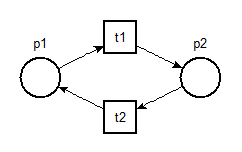
\includegraphics[width=6cm]{./figuras/RDP_SIMPLES.png}\centering
	\fonte{Autoria pr\'opria.}
\end{figure}






Na figura~\ref{fig:esquemaformal} é apresentado uma representa\c{c}\~ao da proposta de desenvolvimento de um projeto, o qual um sistema \'e modelado e ent\~ao a interface, com base na an\'alise do modelo formal, gera um c\'odigo implement\'avel para o controlador selecionado. 

 O esquema est\'a seccionado em sete passos, s\~ao eles:
 
 \begin{itemize}
 	\item Passo 1: Modelagem do sistema f\'isico em Redes de Petri;
 	\item Passo 2: Obten\c{c}\~ao dos aut\^omatos da planta e das especifica\c{c}\~oes;
 	\item Passo 3: Aplica\c{c}\~ao da Teoria de Controle Supervis\'orio;
 	\item Passo 4: Obten\c{c}\~ao do aut\^omato da l\'ogica de controle sintetizada;
 	\item Passo 5: Preparar a l\'ogica de controle para ser convertida;
 	\item Passo 6: Gera\c{c}\~ao do c\'odigo implement\'avel;
 	\item Passo 7: Implementa\c{c}\~ao do c\'odigo em um controlador.
 \end{itemize}

\begin{figure}[!htb]
	%\captionsetup{width=0.97\textwidth}
	\caption[Esquema da abordagem formal para controle de um SED]{Esquema da abordagem formal para controle de um SED.}
	\label{fig:esquemaformal}
	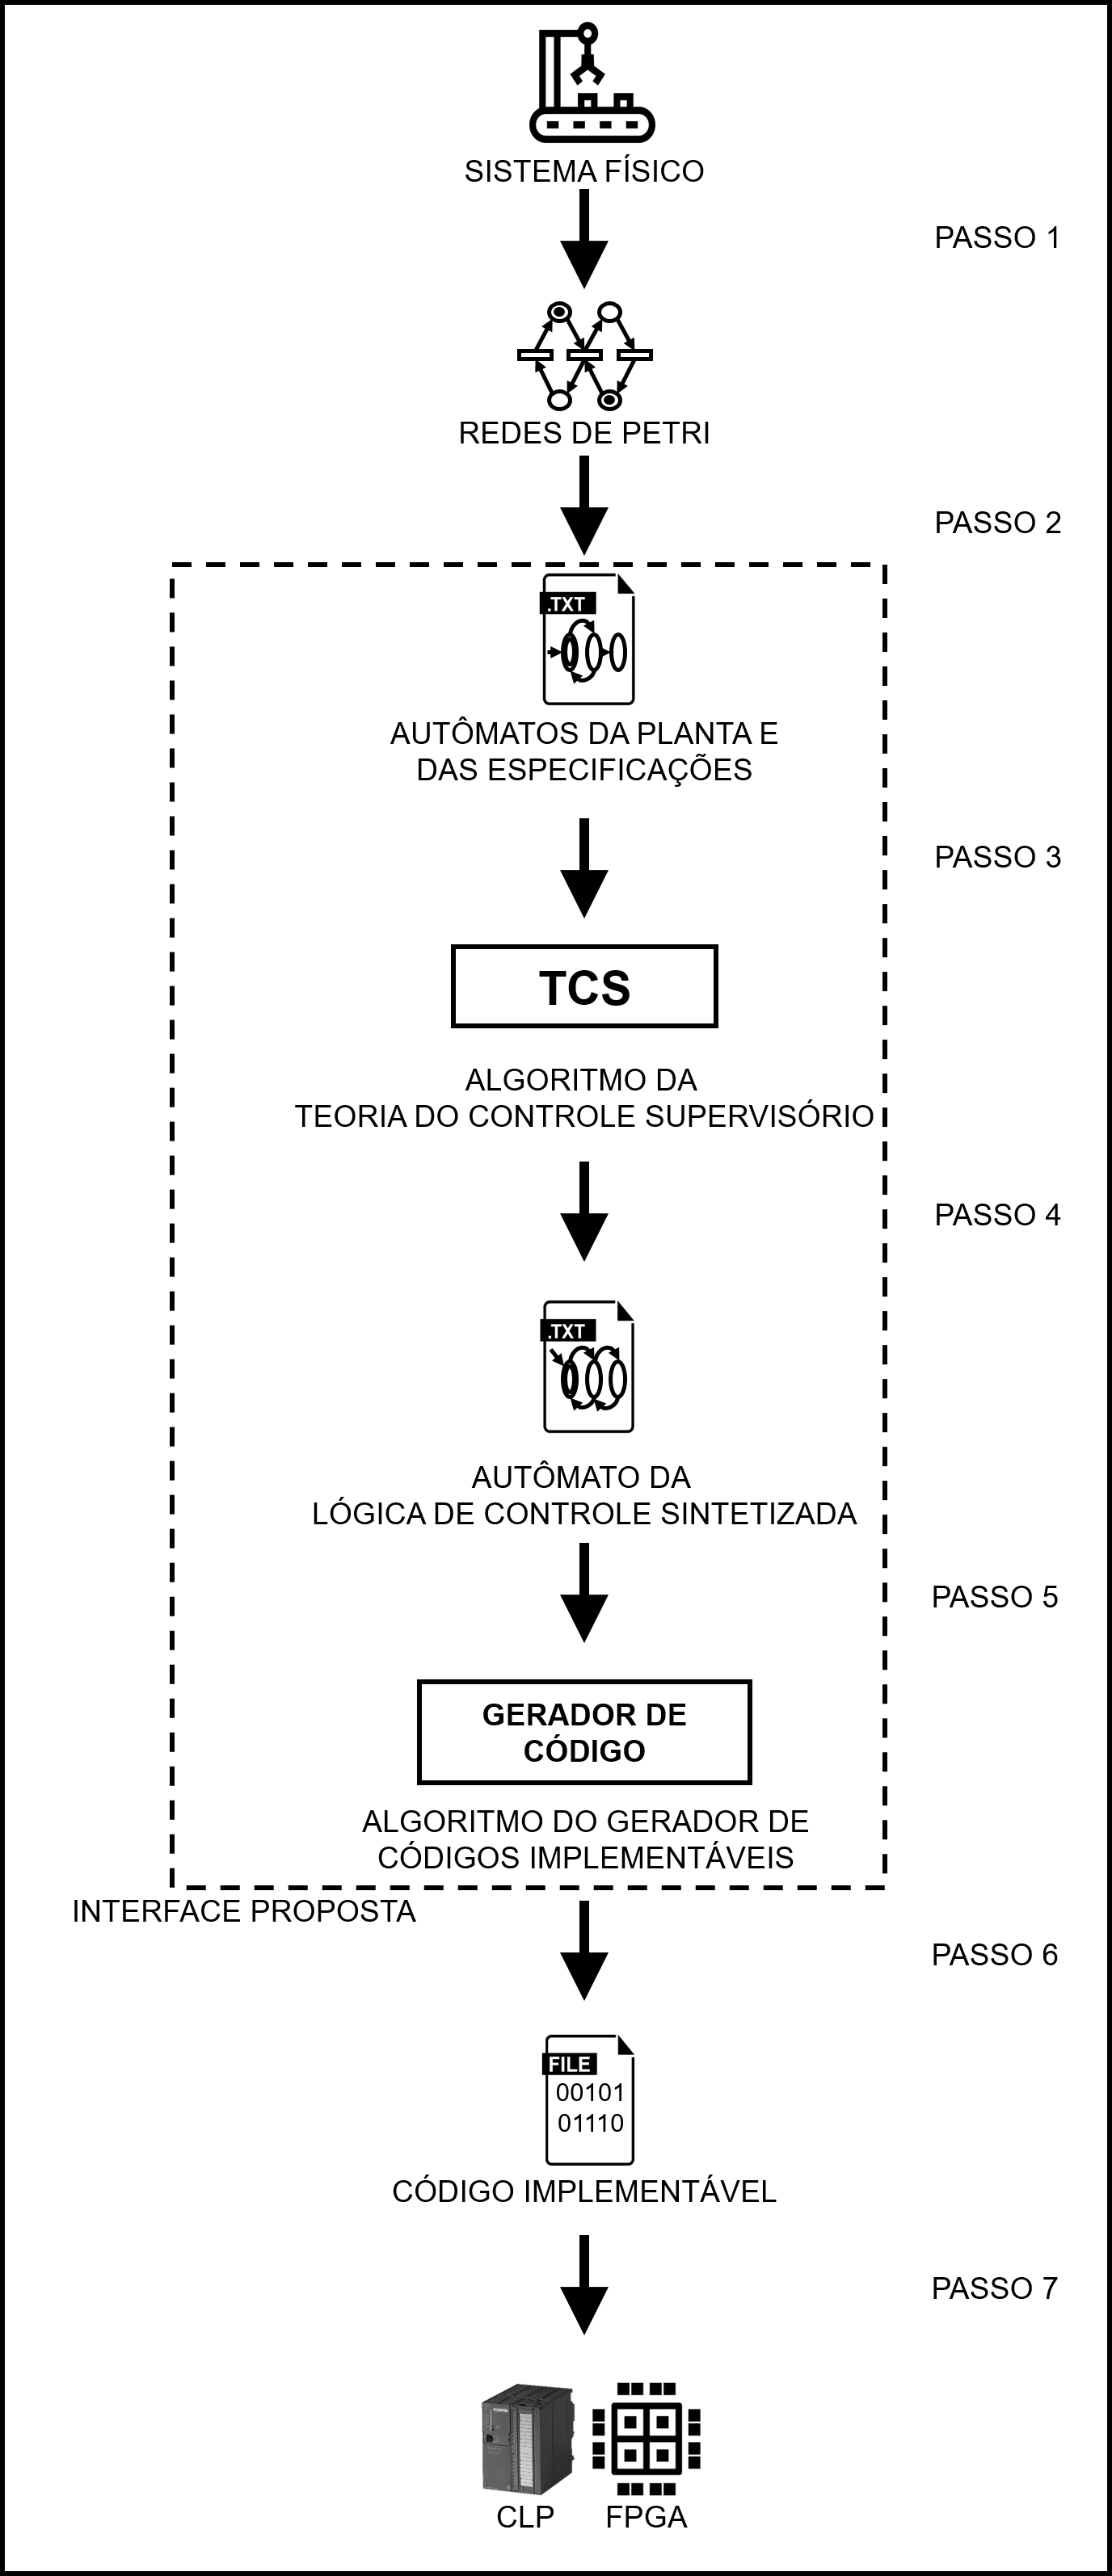
\includegraphics[width=10cm]{./figuras/ESQUEMA_MODELAGEM_FORMAL.png}\centering
	\fonte{Autoria pr\'opria.}
\end{figure}

\subsection{Modelagem do sistema f\'isico em Redes de Petri}


H\'a diversos softwares para modelagem de Redes de Petri, por\'em o software TINA, criado pelo Laborat\'orio de An\'alises e Arquitetura de Sistemas da Universidade de Toulouse, \'e o \'unico que preenche os requisitos para ser executado em conjunto com a interface, gra\c{c}as a formata\c{c}\~ao de seus arquivos de sa\'ida. TINA possui diversas ferramentas para manipular as Redes Petri, tanto para an\'alise quanto para simula\c{c}\~ao. Para este caso a ferramenta de an\'alise de alcan\c{c}abilidade gera para o usu\'ario um arquivo em texto contendo v\'arias informa\c{c}\~oes sobre o grafo de marca\c{c}\~oes.

Neste passo, o usu\'ario modela o sistema f\'isico em Redes de Petri no software TINA.

\subsection{Obten\c{c}\~ao dos aut\^omatos da planta e das especifica\c{c}\~oes}

Uma vez que o sistema foi modelado e analisado, o arquivo oriundo da modelagem do TINA ser\'a carregado na interface, a qual ir\'a rearranjar as informa\c{c}\~oes e dividi-las em m\'aquina de estado finitos devido as marca\c{c}\~oes da rede e demais informa\c{c}\~oes para gerar a especifica\c{c}\~ao do controle supervis\'orio.


\subsection{Aplica\c{c}\~ao da Teoria de Controle Supervis\'orio}

A s\'intese do supervisor \'e realizada para um dado modelo com o objetivo de satisfazer uma especifica\c{c}\~ao de comportamento desejada, onde o supervisor define quais as a\c{c}\~oes de controle que devem ser implementadas \cite{Montgomery2004}.

No caso do algoritmo para aplicar a TCS, se destacam os softwares UMDES \cite{umdes}, desenvolvida pela Universidade de Michigan nos Estados Unidos, e o IDES \cite{ides}, desenvolvida pela Universidade de Queen no Canad\'a. Estes software proporcionam uma f\'acil aplica\c{c}\~ao da TCS partindo de dois aut\^omatos: a planta e as especifica\c{c}\~oes.

\subsection{Obten\c{c}\~ao do aut\^omato da l\'ogica de controle sintetizada}

Neste passo do processo a interface recarrega os aut\^omatos produzidos pelos softwares indicados no item anterior.

\subsection{Preparar a l\'ogica de controle para ser convertida}

A l\'ogica de controle s\'intetizada em forma de aut\^omato \'e formatada para agregar as informa\c{c}\~oes rotuladas durante a modelagem do sistema, essas informa\c{c}\~oes permitem que o c\'odigo a ser gerado contenha os mesmos r\'otulos criado pelo usu\'ario. 

\subsection{Gera\c{c}\~ao do c\'odigo implement\'avel}

A gera\c{c}\~ao dos c\'odigos implement\'aveis ser\'a feita, inspirada nos trabalhos de \cite{hugomestrado} e \cite{disc}, a partir da compara\c{c}\~ao de similaridade da estrutura da l\'ogica sintetizada e a linguagem de programa\c{c}\~ao escolhida.

A programa\c{c}\~ao de controladores l\'ogico program\'aveis em \textit{Sequential Function Chart} (SFC) tem estrutura baseada no \textit{Grafcet}, que por sua vez evoluiu da Redes de Petri, \cite{Martin1999}. Assim, a l\'ogica de controle ser\'a convertida para Redes de Petri e finalmente usada para gerar um arquivo implement\'avel para CLPs em programa\c{c}\~ao SFC.

A gera\c{c}\~ao dos c\'odigos implement\'aveis para FPGAs ser\'a mais simples, pois sua estrutura de programa\c{c}\~ao \textit{VHDL}, uma linguagem de programa\c{c}\~ao de \textit{hardware}, pode ser estruturada como m\'aquina de estados finitos que combina com o aut\^omato sintetizado.

\subsection{Implementa\c{c}\~ao do c\'odigo em um controlador}

O c\'odigo est\'a pronto para ser carregado no controlador selecionado com garantia de controle \'otimo devido ao uso da abordagem formal.

%%%%%%%%%%%%%%%%%%%%%%%



%
%Inserir FIGURA sobre a INTERFACE

%\begin{figure}[!htb]
	%\captionsetup{width=0.97\textwidth}
%	\caption[Esquema dos subsistemas da interface]{Esquema dos subsistemas da interface.}
%	\label{fig:interface}
%	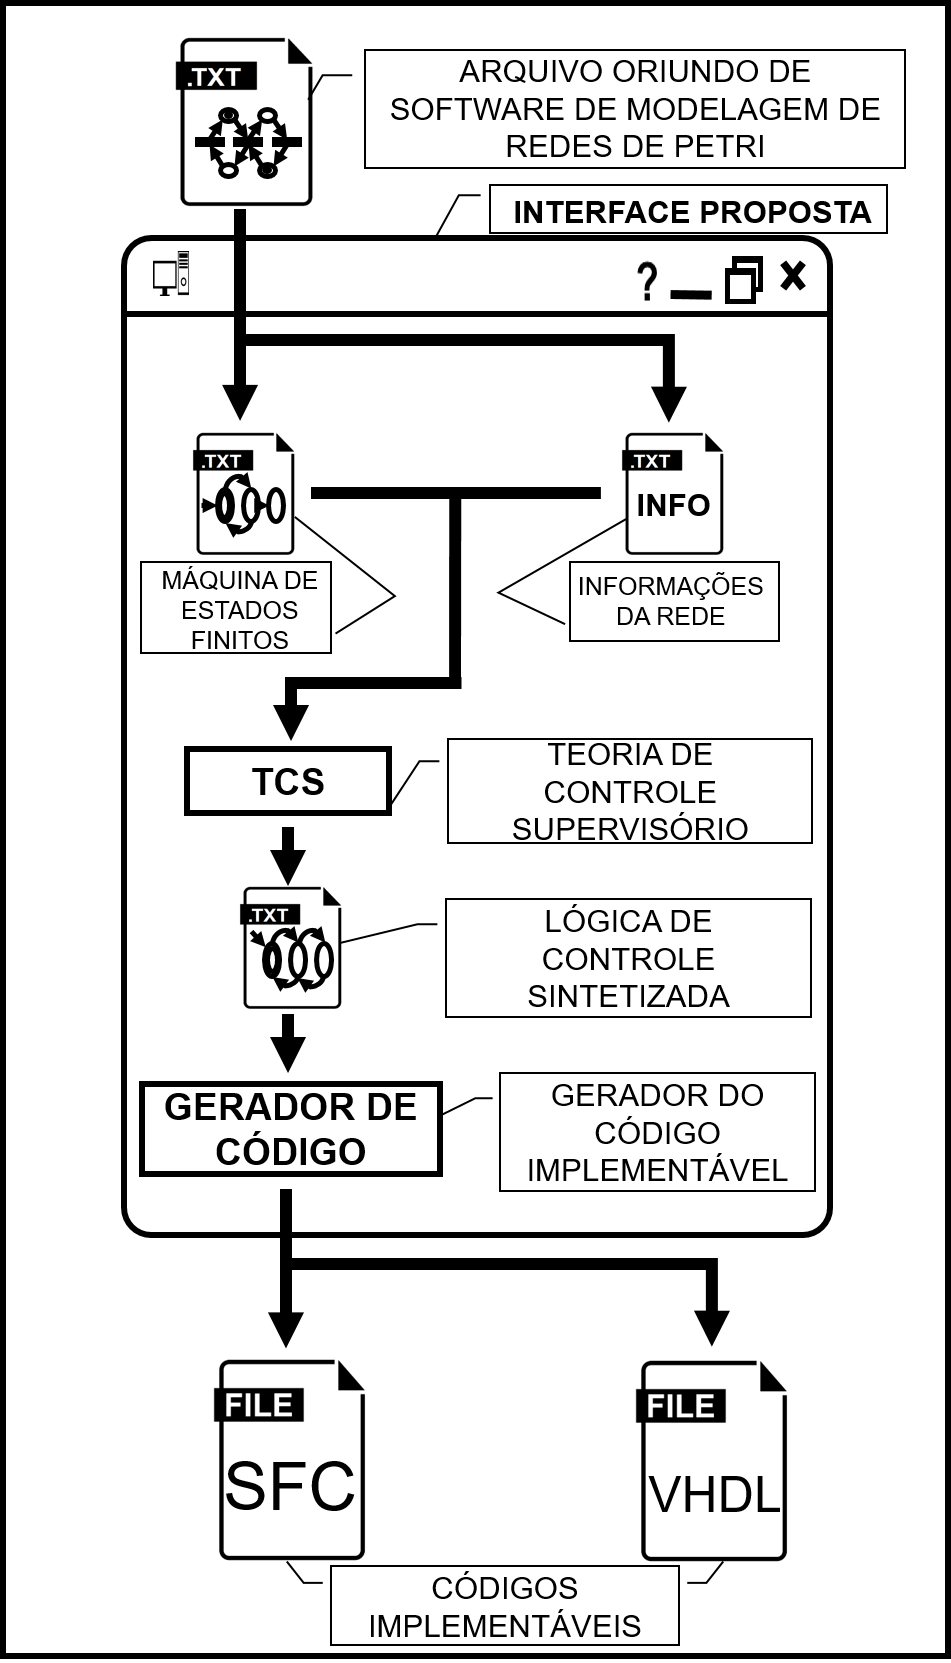
\includegraphics[width=12cm]{./figuras/ESQUEMA_INTERFACE.png}\centering
%	\fonte{Autoria pr\'opria}
%\end{figure}

%H\'a diversos softwares para realizar modelagem e an\'alise de Redes de Petri. Um desses \'e TINA, criado pelo Laborat\'orio de An\'alises e Arquitetura de Sistemas da Universidade de Toulouse. TINA \'e um software de uso livre, e se destaca por possuir uma fun\c{c}\~ao a qual exporta em arquivo de texto as propriedades da rede modelada. Uma das propriedades \'e o grafo, ou \'arvore, de alcan\c{c}abilidade de uma RdP a qual representa todos os estados alcan\c{c}\'aveis e \'e representado por um aut\^omato finito.
%O usu\'ario precisar\'a seguir certas regras ao modelar um sistema, como a rotula\c{c}\~ao de eventos e transi\c{c}\~oes, para que o programa interprete de forma correta as informa\c{c}\~oes. Essas regras estar\~ao presentes na interface do software, bem como um tutorial.

%A partir do grafo de alcan\c{c}abilidade convertido do formato padr\~ao do TINA para o formato de m\'aquina de estados finito, este poder\'a ser executado por outro software para aplicar o Teorema do Controle Supervi\'osio e gerar um aut\^omato supervisor. Entre os softwares que implementam o teorema, se destacam o UMDES, desenvolvida pela Universidade de Michigan, e o IDES, desenvolvida pela Universidade de Queen. A convers\~ao ter\'a base nas informa\c{c}\~oes adicionais, como por exemplo se um evento \'e control\'avel ou somente observ\'avel. O resultado deste processo ser\'a o supervisor do sistema.

%Com o supervisor pronto, o pr\'oximo passo \'e a gera\c{c}\~ao do c\'odigo implement\'avel, este ser\'a realizado seguindo a norma IEC 61131-3, uma norma que rege o padr\~ao de linguagens de programa\c{c}\~ao de controladores l\'ogico program\'aveis, e tamb\'em a norma IEEE 1076, a qual rege a linguagem de descri\c{c}\~ao de hardware VHDL para FPGAs. O programa interpretar\'a o supervisor e ir\'a transcrever este na forma de linhas de c\'odigos. O processo resultar\'a em arquivos pronto para serem embarcados nos sistemas mencionados.




%PROPOSTA

\chapter{Automa\c{c}\~ao Industrial}

Neste cap\'itulo ser\'a abordado dois cen\'arios para apresentar a proposta. O primeiro cen\'ario discute o modo usual de implementar um controlador atrav\'es de uma abordagem informal. No segundo cen\'ario ser\'a apresentado uma proposta para a implementa\c{c}\~ao de um controlador utilizando uma abordagem formal.

\section{M\'etodo informal}

Na figura~\ref{fig:esquemainformal} \'e mostrado o esquema da solu\c{c}\~ao usual de automa\c{c}\~ao de um sistema.

Neste cen\'ario, o usu\'ario deduz uma solu\c{c}\~ao para o problema de controle. Uma solu\c{c}\~ao obtida empiricamente pode resultar numa l\'ogica de controle falha, a qual pode colocar em risco a seguran\c{c}a do sistema. A verifica\c{c}\~ao do controle nesse caso \'e via tentativa e erro o que estende o tempo de projeto.

\begin{figure}[!htb]
	%\captionsetup{width=0.97\textwidth}
	\caption[Esquema da abordagem informal para controle de um SED]{Esquema da abordagem informal para controle de um SED.}
	\label{fig:esquemainformal}
	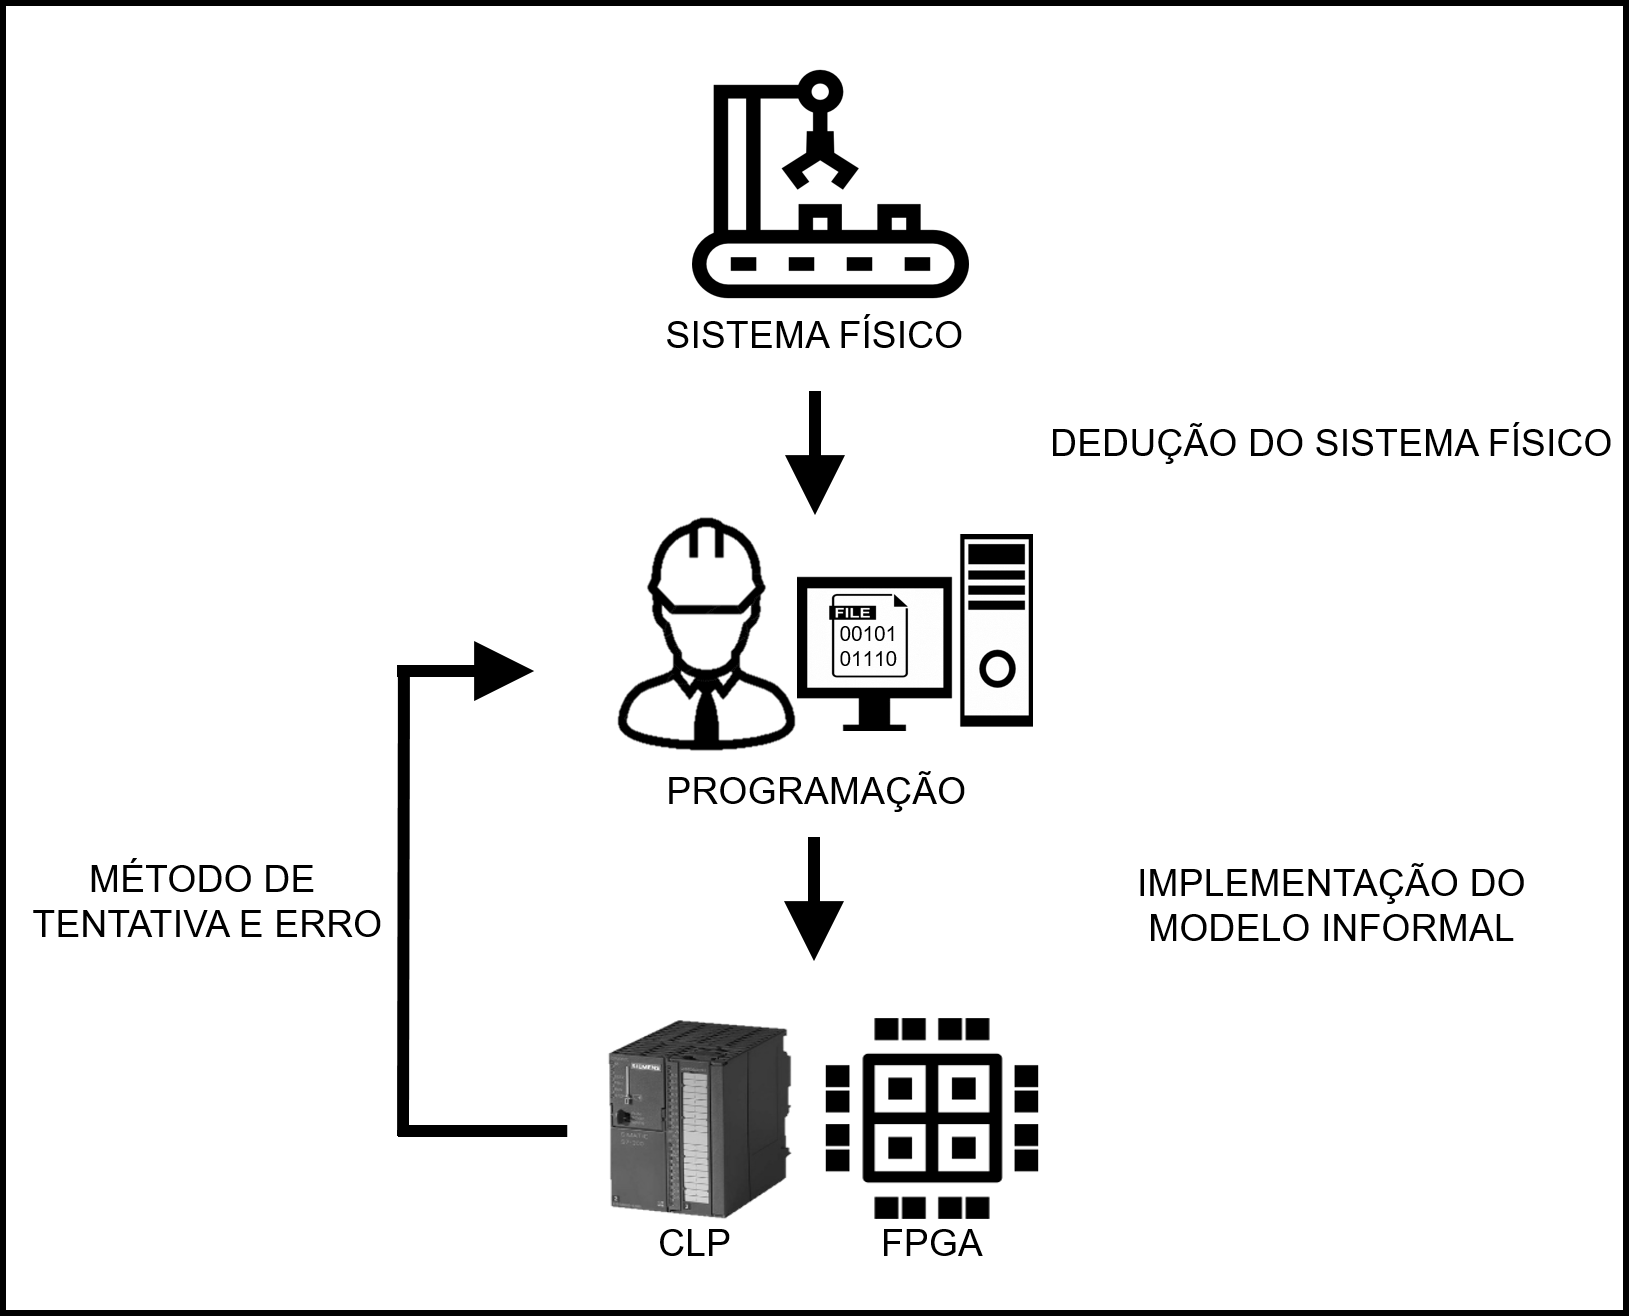
\includegraphics[width=16cm]{./figuras/ESQUEMA_MODELAGEM_INFORMAL.png}\centering
	\fonte{Autoria pr\'opria.}
\end{figure}

\section{M\'etodo formal}

Na figura~\ref{fig:esquemaformal} é apresentado uma representa\c{c}\~ao da proposta de desenvolvimento de um projeto, o qual um sistema \'e modelado e ent\~ao a interface, com base na an\'alise do modelo formal, gera um c\'odigo implement\'avel para o controlador selecionado. 

 O esquema est\'a seccionado em sete passos, s\~ao eles:
 
 \begin{itemize}
 	\item Passo 1: Modelagem do sistema f\'isico em Redes de Petri;
 	\item Passo 2: Obten\c{c}\~ao dos aut\^omatos da planta e das especifica\c{c}\~oes;
 	\item Passo 3: Aplica\c{c}\~ao da Teoria de Controle Supervis\'orio;
 	\item Passo 4: Obten\c{c}\~ao do aut\^omato da l\'ogica de controle sintetizada;
 	\item Passo 5: Preparar a l\'ogica de controle para ser convertida;
 	\item Passo 6: Gera\c{c}\~ao do c\'odigo implement\'avel;
 	\item Passo 7: Implementa\c{c}\~ao do c\'odigo em um controlador.
 \end{itemize}

\begin{figure}[!htb]
	%\captionsetup{width=0.97\textwidth}
	\caption[Esquema da abordagem formal para controle de um SED]{Esquema da abordagem formal para controle de um SED.}
	\label{fig:esquemaformal}
	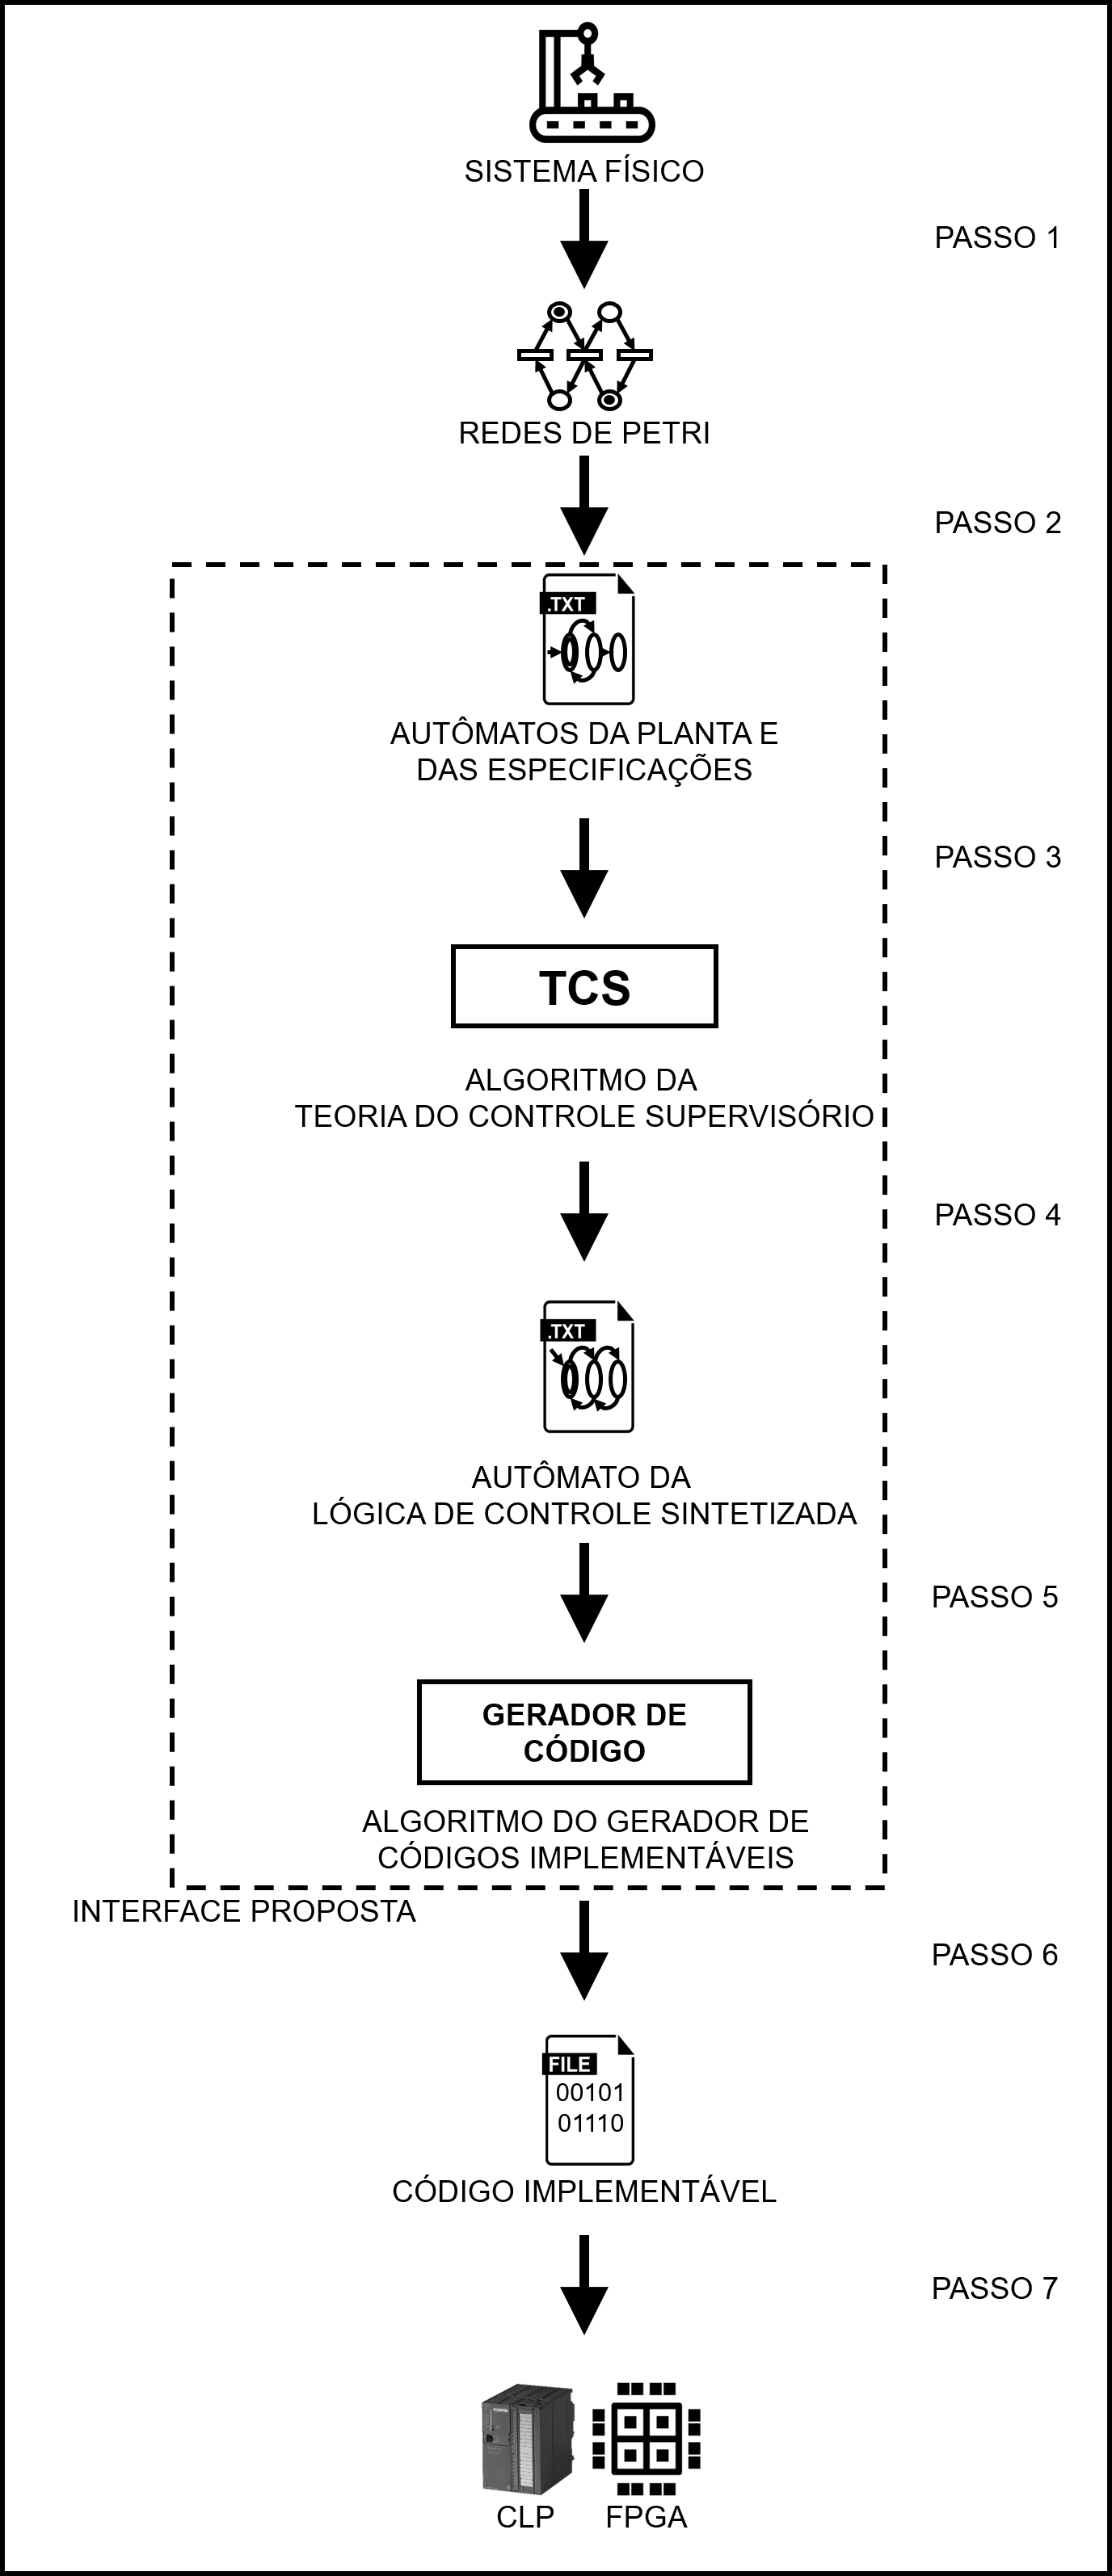
\includegraphics[width=10cm]{./figuras/ESQUEMA_MODELAGEM_FORMAL.png}\centering
	\fonte{Autoria pr\'opria.}
\end{figure}

\subsection{Modelagem do sistema f\'isico em Redes de Petri}


H\'a diversos softwares para modelagem de Redes de Petri, por\'em o software TINA, criado pelo Laborat\'orio de An\'alises e Arquitetura de Sistemas da Universidade de Toulouse, \'e o \'unico que preenche os requisitos para ser executado em conjunto com a interface, gra\c{c}as a formata\c{c}\~ao de seus arquivos de sa\'ida. TINA possui diversas ferramentas para manipular as Redes Petri, tanto para an\'alise quanto para simula\c{c}\~ao. Para este caso a ferramenta de an\'alise de alcan\c{c}abilidade gera para o usu\'ario um arquivo em texto contendo v\'arias informa\c{c}\~oes sobre o grafo de marca\c{c}\~oes.

Neste passo, o usu\'ario modela o sistema f\'isico em Redes de Petri no software TINA.

\subsection{Obten\c{c}\~ao dos aut\^omatos da planta e das especifica\c{c}\~oes}

Uma vez que o sistema foi modelado e analisado, o arquivo oriundo da modelagem do TINA ser\'a carregado na interface, a qual ir\'a rearranjar as informa\c{c}\~oes e dividi-las em m\'aquina de estado finitos devido as marca\c{c}\~oes da rede e demais informa\c{c}\~oes para gerar a especifica\c{c}\~ao do controle supervis\'orio.


\subsection{Aplica\c{c}\~ao da Teoria de Controle Supervis\'orio}

A s\'intese do supervisor \'e realizada para um dado modelo com o objetivo de satisfazer uma especifica\c{c}\~ao de comportamento desejada, onde o supervisor define quais as a\c{c}\~oes de controle que devem ser implementadas \cite{Montgomery2004}.

No caso do algoritmo para aplicar a TCS, se destacam os softwares UMDES \cite{umdes}, desenvolvida pela Universidade de Michigan nos Estados Unidos, e o IDES \cite{ides}, desenvolvida pela Universidade de Queen no Canad\'a. Estes software proporcionam uma f\'acil aplica\c{c}\~ao da TCS partindo de dois aut\^omatos: a planta e as especifica\c{c}\~oes.

\subsection{Obten\c{c}\~ao do aut\^omato da l\'ogica de controle sintetizada}

Neste passo do processo a interface recarrega os aut\^omatos produzidos pelos softwares indicados no item anterior.

\subsection{Preparar a l\'ogica de controle para ser convertida}

A l\'ogica de controle s\'intetizada em forma de aut\^omato \'e formatada para agregar as informa\c{c}\~oes rotuladas durante a modelagem do sistema, essas informa\c{c}\~oes permitem que o c\'odigo a ser gerado contenha os mesmos r\'otulos criado pelo usu\'ario. 

\subsection{Gera\c{c}\~ao do c\'odigo implement\'avel}

A gera\c{c}\~ao dos c\'odigos implement\'aveis ser\'a feita, inspirada nos trabalhos de \cite{hugomestrado} e \cite{disc}, a partir da compara\c{c}\~ao de similaridade da estrutura da l\'ogica sintetizada e a linguagem de programa\c{c}\~ao escolhida.

A programa\c{c}\~ao de controladores l\'ogico program\'aveis em \textit{Sequential Function Chart} (SFC) tem estrutura baseada no \textit{Grafcet}, que por sua vez evoluiu da Redes de Petri, \cite{Martin1999}. Assim, a l\'ogica de controle ser\'a convertida para Redes de Petri e finalmente usada para gerar um arquivo implement\'avel para CLPs em programa\c{c}\~ao SFC.

A gera\c{c}\~ao dos c\'odigos implement\'aveis para FPGAs ser\'a mais simples, pois sua estrutura de programa\c{c}\~ao \textit{VHDL}, uma linguagem de programa\c{c}\~ao de \textit{hardware}, pode ser estruturada como m\'aquina de estados finitos que combina com o aut\^omato sintetizado.

\subsection{Implementa\c{c}\~ao do c\'odigo em um controlador}

O c\'odigo est\'a pronto para ser carregado no controlador selecionado com garantia de controle \'otimo devido ao uso da abordagem formal.

%%%%%%%%%%%%%%%%%%%%%%%



%
%Inserir FIGURA sobre a INTERFACE

%\begin{figure}[!htb]
	%\captionsetup{width=0.97\textwidth}
%	\caption[Esquema dos subsistemas da interface]{Esquema dos subsistemas da interface.}
%	\label{fig:interface}
%	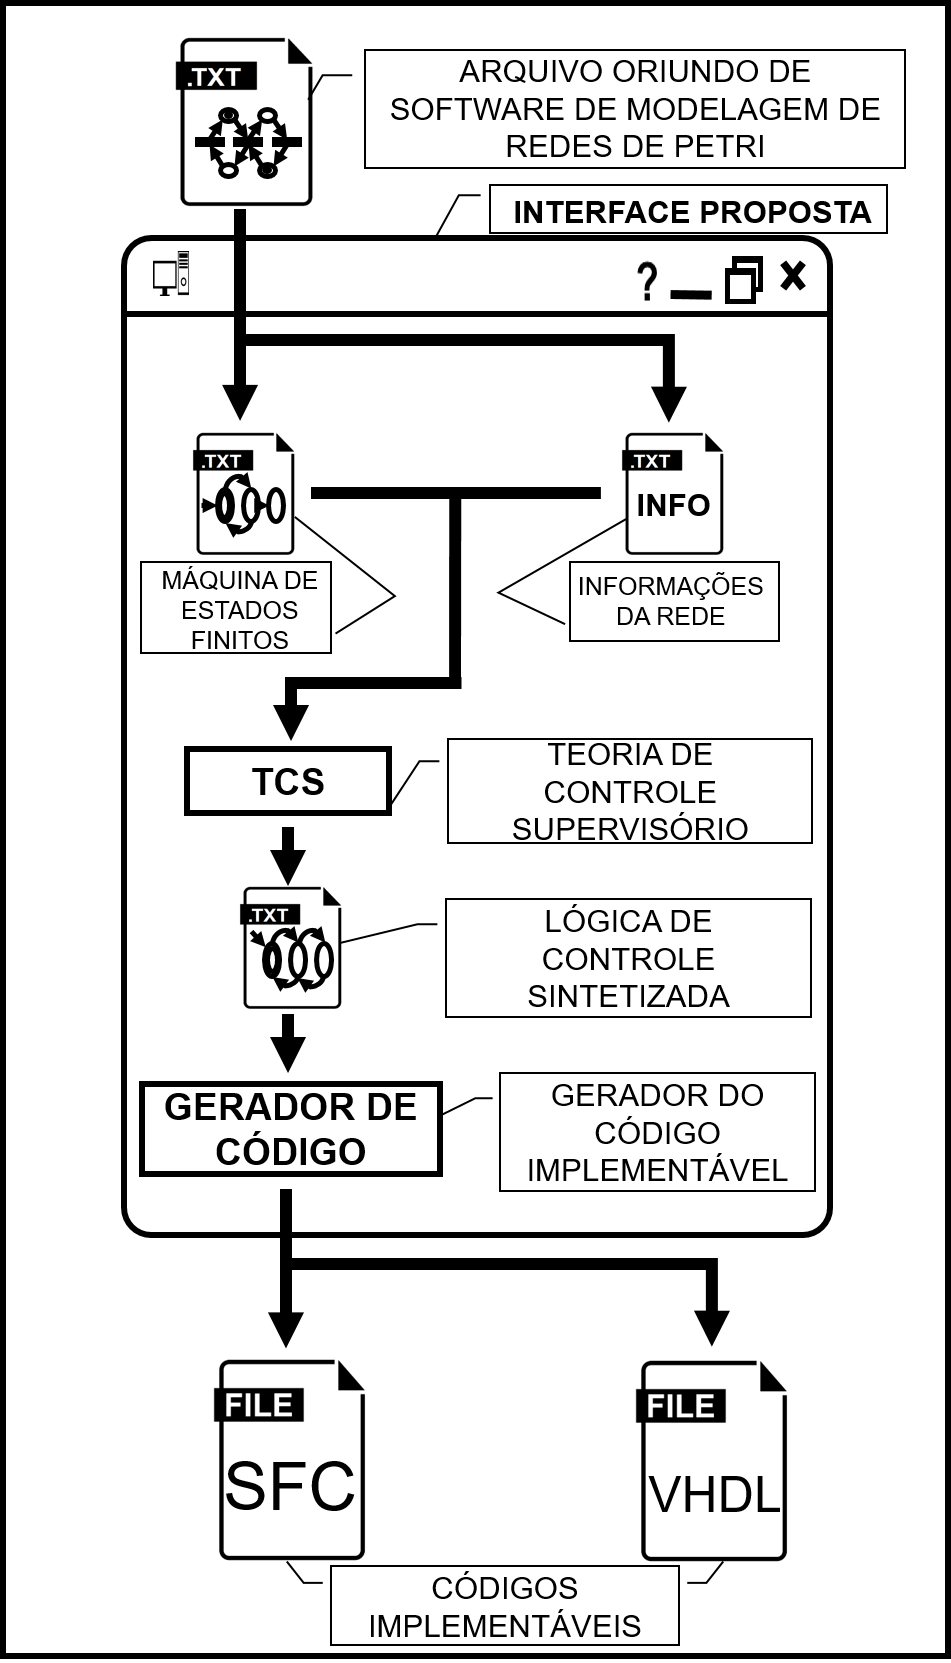
\includegraphics[width=12cm]{./figuras/ESQUEMA_INTERFACE.png}\centering
%	\fonte{Autoria pr\'opria}
%\end{figure}

%H\'a diversos softwares para realizar modelagem e an\'alise de Redes de Petri. Um desses \'e TINA, criado pelo Laborat\'orio de An\'alises e Arquitetura de Sistemas da Universidade de Toulouse. TINA \'e um software de uso livre, e se destaca por possuir uma fun\c{c}\~ao a qual exporta em arquivo de texto as propriedades da rede modelada. Uma das propriedades \'e o grafo, ou \'arvore, de alcan\c{c}abilidade de uma RdP a qual representa todos os estados alcan\c{c}\'aveis e \'e representado por um aut\^omato finito.
%O usu\'ario precisar\'a seguir certas regras ao modelar um sistema, como a rotula\c{c}\~ao de eventos e transi\c{c}\~oes, para que o programa interprete de forma correta as informa\c{c}\~oes. Essas regras estar\~ao presentes na interface do software, bem como um tutorial.

%A partir do grafo de alcan\c{c}abilidade convertido do formato padr\~ao do TINA para o formato de m\'aquina de estados finito, este poder\'a ser executado por outro software para aplicar o Teorema do Controle Supervi\'osio e gerar um aut\^omato supervisor. Entre os softwares que implementam o teorema, se destacam o UMDES, desenvolvida pela Universidade de Michigan, e o IDES, desenvolvida pela Universidade de Queen. A convers\~ao ter\'a base nas informa\c{c}\~oes adicionais, como por exemplo se um evento \'e control\'avel ou somente observ\'avel. O resultado deste processo ser\'a o supervisor do sistema.

%Com o supervisor pronto, o pr\'oximo passo \'e a gera\c{c}\~ao do c\'odigo implement\'avel, este ser\'a realizado seguindo a norma IEC 61131-3, uma norma que rege o padr\~ao de linguagens de programa\c{c}\~ao de controladores l\'ogico program\'aveis, e tamb\'em a norma IEEE 1076, a qual rege a linguagem de descri\c{c}\~ao de hardware VHDL para FPGAs. O programa interpretar\'a o supervisor e ir\'a transcrever este na forma de linhas de c\'odigos. O processo resultar\'a em arquivos pronto para serem embarcados nos sistemas mencionados.




%PROJETO

\chapter{PN2IC}

Neste cap\'itulo ser\'a apresentado a ferramenta PN2IC (Petri Net 2 Implementable Code).

\section{Algoritmo de leitura e aplica\c{c}\~ao do TCS}

O algoritmo de leitura e a aplica\c{c}\~ao do TCS seguem os seguintes passos.
 \begin{itemize}
 	\item Passo 1: Modelagem do sistema em Redes de Petri;
 	\item Passo 2: Inser\c{c}\~ao da modelagem na ferramenta;
 	\item Passo 3: Adi\c{c}\~ao de equa\c{c}\~oes de restri\c{c}\~ao;
 	\item Passo 4: Extra\c{c}\~ao da RdP com o supervis\'orio;
 	\item Passo 5: Avalia\c{c}\~ao das propriedades da RdP na ferramenta de modelagem;
 	\item Passo 6: Execu\c{c}\~ao do conversor para c\'odigo implementa\'el;
 	\item Passo 7: Implementa\c{c}\~ao do c\'odigo em um controlador.
 \end{itemize}


\section{Modelagem do sistema em Redes de Petri}
O usu\'ario dever\'a modelar a planta em uma ferramenta que permita a exporta\c{c}\~ao do modelo em formato PNML (Petri Net Markup Language). Esse formato \'e regido pela ISO/IEC 15909-3, e utiliza como base a linguagem de marca\c{c}\~ao XML (eXtensible Markup Language) afim de padronizar um formato de arquivo para a RdP \cite{pnmlorg}. No ap\^endice ?? \'e apresentado a estrutura b\'asica de um arquivo PNML.

\section{Interface gr\'afica}
A interface gr\'afica tem por objetivo facilitar as entradas de dados pelo usu\'ario. Nela o usu\'ario indica o arquivo PNML, adiciona as especifica\c{c}\~oes da planta e gera os arquivos da nova RdP e o c\'odigo implement\'avel. 

Na figura~\ref{fig:interfacegrafica} \'e apresentado a interface gr\'afica.

\begin{figure}[!htb]
	%\captionsetup{width=0.97\textwidth}
	\caption[Interface gr\'afica do projeto PN2IC.]{Interface gr\'afica do projeto PN2IC.}
	\label{fig:interfacegrafica}
	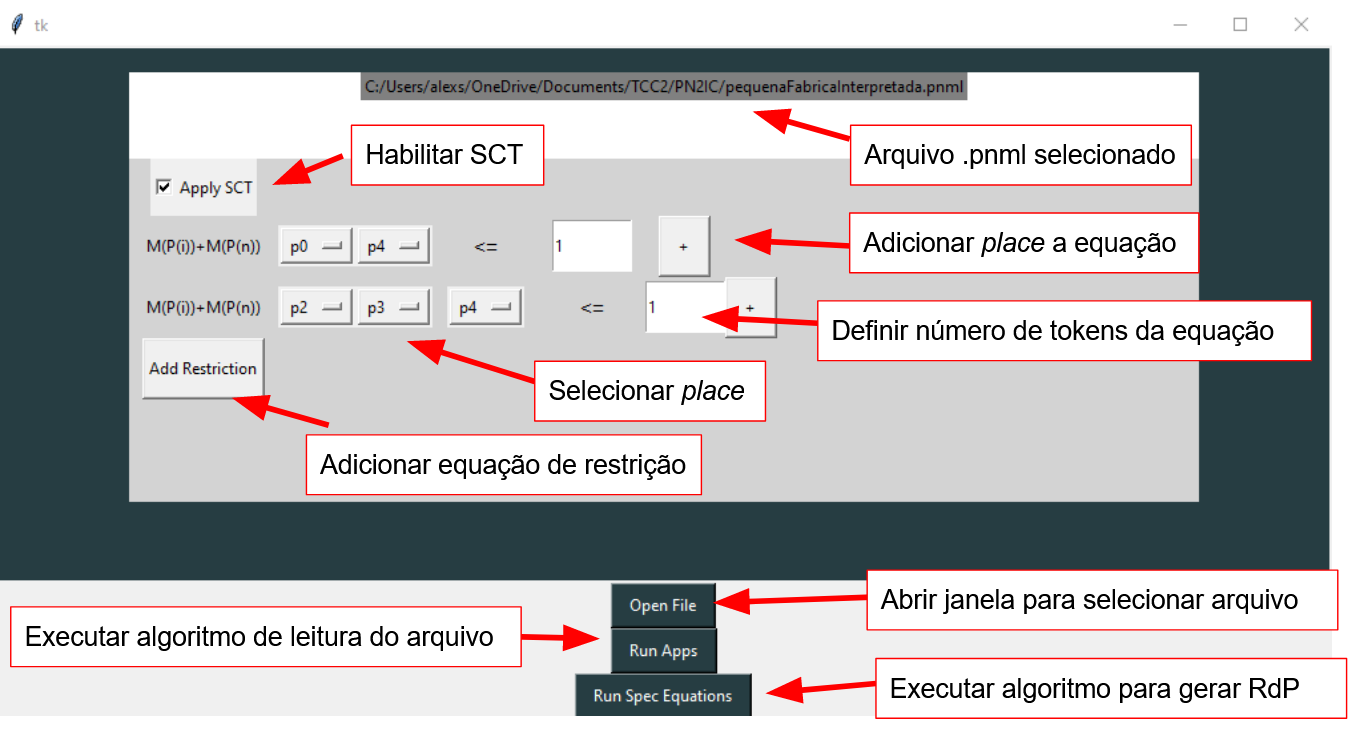
\includegraphics[width=16cm]{./figuras/INTERFACE_GRAFICA_PN2IC.png}\centering
	\fonte{Autoria pr\'opria.}
\end{figure}

\section{Extra\c{c}\~ao das informa\c{c}\~oes da RdP}
Ap\'os a escolha do arquivo PNML pelo usu\'ario, a ferramenta executa uma extra\c{c}\~ao de informa\c{c}\~oes da RdP e armazena de forma orientada a objetos. Para isso, foi criado tr\^es classes; Place, Transition e Arc. Cada classe de objeto representa um elemento da rede, Place representa o Lugar e tem como propriedade seu c\'odigo identidade, nome, r\'otulo e se h\'a marca\c{c}\~ao inicial. Transition tamb\'em possui propriedades como identidade, nome e r\'otulo.
O caso mais especial \'e da classe Arc, que \'e o arco que interliga os elementos de uma RdP. Arc possui como propriedades a sua identidade, a fonte de onde parte o arco e o seu alvo onde termina o arco. Tamb\'em possui m\'etodos de classe que retornam uma lista de transi\c{c}\~oes dado uma identidade de um Lugar, s\~ao duas fun\c{c}\~oes que retornam transi\c{c}\~oes que precedem ou sucedem dado Lugar. As propriedades das classes s\~ao ilustradas na figura~\ref{fig:classes}.

\begin{figure}[!htb]
	%\captionsetup{width=0.97\textwidth}
	\caption[Classes de objetos participantes da RdP.]{Classes de objetos participantes da RdP.}
	\label{fig:classes}
	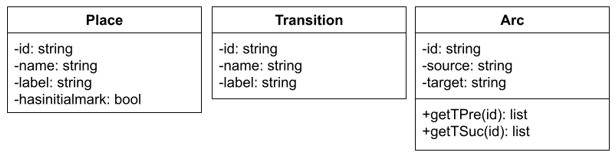
\includegraphics[width=16cm]{./figuras/CLASSES.png}\centering
	\fonte{Autoria pr\'opria.}
\end{figure}

\section{Abordagem h\'ibrida de Uzam e Wonham}

No trabalho \cite{UzamWonham2005}, \'e apresentado uma abordagem h\'ibrida para o controle supervis\'orio de SEDs atrav\'es do acoplamento de supervis\'orios RW (Ramadge Wonham) em Redes de Petri. Este trabalho consiste em simplificar uma RdP, de um modelo n\~ao control\'avel, e representar a rede e sua especifica\c{c}\~ao, que \'e um conjunto de estados proibidos, em aut\^omatos e ent\~ao aplicar a TCS para obter o supervis\'orio RW. O supervis\'orio RW \'e respresentado em RdP passando a se chamar auto-net e este \'e acoplado no modelo inicial n\~ao control\'avel. Na ~\ref{fig:uzamcontrol} \'e apresentado a abordagem h\'ibrida de um controle supervis\'orio de uma RdP.

\begin{figure}[!htb]
	%\captionsetup{width=0.97\textwidth}
	\caption[Controle supervis\'orio de um SED baseado na abordagem de \cite{UzamWonham2005}.]{Controle supervis\'orio de um SED baseado na abordagem de \cite{UzamWonham2005}.}
	\label{fig:uzamcontrol}
	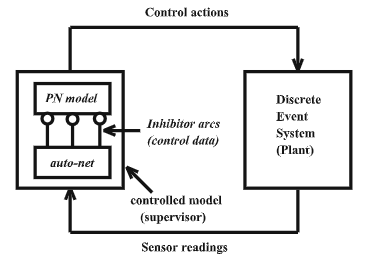
\includegraphics[width=16cm]{./figuras/UZAMCONTROL.png}\centering
	\fonte{\cite{UzamWonham2005}}
\end{figure}



\section{Abordagem aplicada no projeto}

Neste projeto, a metodologia aplicada \'e baseada na abordadem h\'ibrida de \cite{UzamWonham2005}. As diferen\c{c}as ficam por conta da n\~ao simplifica\c{c}\~ao da RdP inicial e a n\~ao utiliza\c{c}\~ao do m\'etodo supervisor\'orio RW.

Inspirado no exemplo pequena f\'abrica de \cite{apostilacury}, na figura ~\ref{fig:pqnafab} \'e apresentado uma modelagem em RdP que representa uma pequena f\'abrica. O conjunto de lugares p0 e p1 representam uma c\'elula de usinagem, p4 um buffer (fila) e o conjunto p2 e p3 uma c\'elula de pintura. Um CLP ir\'a comandar a atua\c{c}\~ao das c\'elulas de fabrica\c{c}\~ao e para isso uma l\'ogica discreta e sequencial deve ser desenvolvida, a l\'ogica dever\'a contar com intertravamentos para garantir que, por exemplo, um operador for\c{c}e a atua\c{c}\~ao atrav\'es de comando manual. Esse intertravamento \'e o que comp\~oe o sistema de supervis\~ao.
As fichas (tokens) em p1 representam ociosidade da usinagem, j\'a em p0 representam o trabalho de usinagem. Em p4 representam pe\c{c}as em aguardo e em p3 ociosidade na pintura e p2 em trabalho de pintura.\

\begin{figure}[!htb]
	%\captionsetup{width=0.97\textwidth}
	\caption[Modelagem de uma pequena f\'abrica.]{Modelagem de uma pequena f\'abrica.}
	\label{fig:pqnafab}
	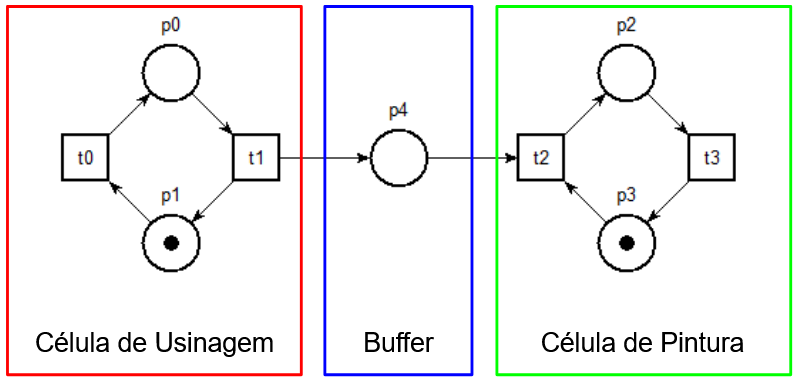
\includegraphics[width=16cm]{./figuras/PQNAFAB.png}\centering
	\fonte{Autoria pr\'opria.}
\end{figure}

A especifica\c{c}\~ao deste projeto \'e que n\~ao haja overflow (ac\'umulo de pe\c{c}as pela c\'elula de usinagem) e nem underflow (in\'icio do processo de pintura sem pe\c{c}as dispon\'iveis) no buffer. Pela pr\'opria propriedade da RdP, em permitir o disparo das transi\c{c}\~oes somente quando os lugares que precedem as transi\c{c}\~oes possuem marca\c{c}\~ao maior ou igual ao peso do arco, \'e impedido o disparo de t2 sem que haja pe\c{c}a em p4. O overflow ficar\'a por conta de um supervisor. Sendo t0 uma transi\c{c}\~ao contro\'avel e t1 um sinal de finaliza\c{c}\~ao do trabalho de usinagem, se faz necess\'ario impedir que a c\'elula de usinagem inicie seu processo quando h\'a pe\c{c}a em p4, sendo assim, a equa\c{c}\~ao da especifica\c{c}\~ao \'e M(p0) + M(p4) <= 1. A soma das fichas de p0 e p4 sempre deve ser menor ou igual a zero, com essa essa especifica\c{c}\~ao garante-se o intertravamento de t0 inibindo o overflow de p4.

Na ferramenta, o usu\'ario seleciona o arquivo de modelagem e preenche a especifica\c{c}\~ao, como mostrado na figura ~\ref{fig:pqnafabentrada}. O algoritmo, partindo do modelo auto\^omato da especifica\c{c}\~ao e seguindo o m\'etodo de \cite{UzamWonham2005}, gera um par de lugares do supervisor com as transi\c{c}\~oes que precedem e sucedem os lugares da especifica\c{c}\~ao.

\begin{figure}[!htb]
	%\captionsetup{width=0.97\textwidth}
	\caption[Entrada de dados da modelagem de uma pequena f\'abrica.]{Entrada de dados da modelagem de uma pequena f\'abrica.}
	\label{fig:pqnafabentrada}
	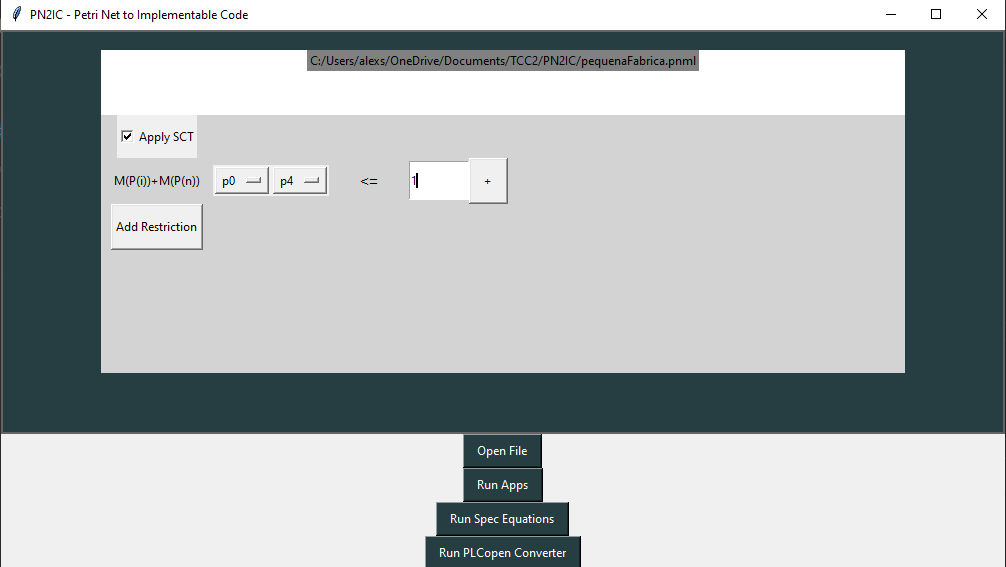
\includegraphics[width=16cm]{./figuras/PQNAFABENTRADA.png}\centering
	\fonte{Autoria pr\'opria.}
\end{figure}

Na figura ~\ref{fig:pqnafabespec} \'e apresentado a convers\~ao da especifica\c{c}\~ao em aut\^omato junto com o par de lugares do supervisor. 

\begin{figure}[!htb]
	%\captionsetup{width=0.97\textwidth}
	\caption[Autômato e RdP resultantes da especifica\c{c}\~ao.]{Autômato e RdP resultantes da especifica\c{c}\~ao.}
	\label{fig:pqnafabespec}
	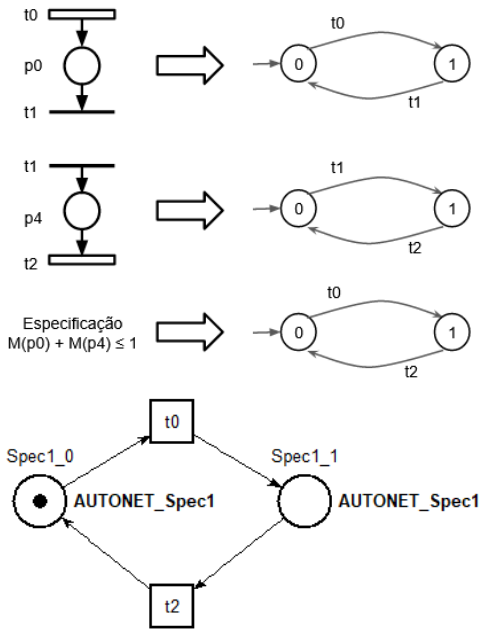
\includegraphics[width=16cm]{./figuras/PQNAFABESPEC.png}\centering
	\fonte{Autoria pr\'opria.}
\end{figure}

O pr\'oximo passo do algoritmo \'e acoplar o supervisor \`a modelagem original. A modelagem com o supervis\'orio \'e mostrado na figura ~\ref{fig:pqnafabsup}.

\begin{figure}[!htb]
	%\captionsetup{width=0.97\textwidth}
	\caption[RdP com o supervisor acoplado.]{RdP com o supervisor acoplado.}
	\label{fig:pqnafabsup}
	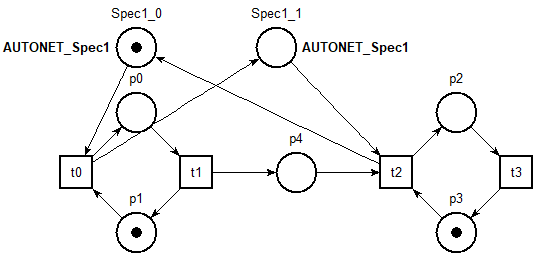
\includegraphics[width=16cm]{./figuras/PQNAFABSUP.png}\centering
	\fonte{Autoria pr\'opria.}
\end{figure}

A modelagem com o supervisor atende os requisitos para uma Rede de Petri limitada, viva e revers\'ivel.

\section{Algoritmo de covers\~ao da Rede de Petri para c\'odigo implementa\'avel}

Duas informa\c{c}\~oes s\~ao necess\'arias para gerar o c\'odigo implement\'avel, a estrutura da RdP e a an\'alise estrutural sobre a invariante de lugar. O algoritmo de extra\c{c}\~ao da RdP \'e o mesmo utilizado na primeira parte do projeto. A informa\c{c}\~ao sobre a invariante de lugar da RdP deve ser extra\'ida na ferramenta TINA. Na figura ~\ref{fig:pqnafabstruct} \'e apresentado a an\'alise dos invariantes de lugar com a RdP em destaque. As invariantes ser\~ao chamadas de flow pois apresentam o fluxo que as fichas percorrem durantes os disparos das transi\c{c}\~oes, cada flow ser\'a uma programa\c{c}\~ao em Sequential Function Chart (SFC).

\begin{figure}[!htb]
	%\captionsetup{width=0.97\textwidth}
	\caption[Invariantes de lugar.]{Invariantes de lugar.}
	\label{fig:pqnafabstruct}
	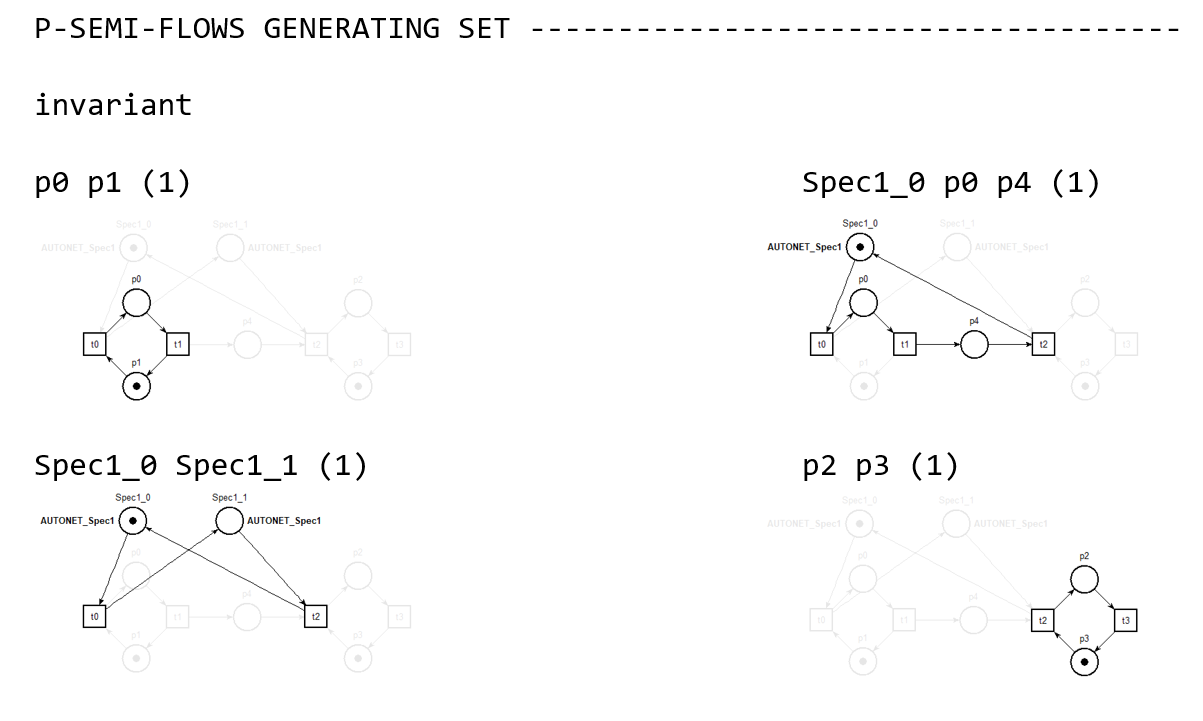
\includegraphics[width=16cm]{./figuras/PQNAFABSTRUCT.png}\centering
	\fonte{Autoria pr\'opria.}
\end{figure}

O algoritmo, com base nos dados fornecidos, define os elementos das Sequential Funtion Charts, como os Steps que representam Lugares, Transitions que representam Transi\c{c}\~oes e InVars e Branches que representam os Arcos de uma RdP. Tamb\'em \'e definido a sequ\^encia de cada elemento e uma SFC somente para definir as transi\c{c}\~oes e sua condi\c{c}\~ao de disparo.

O c\'odigo implement\'avel \'e estruturado no padr\~ao PLCopen. Fundado em 1992, logo ap\'os a padroniza\c{c}\~ao das linguagens de programa\c{c}\~ao de controladores l\'ogico program\'aveis pela IEC 61131-3, PLCopen \'e uma organiza\c{c}\~ao que visa a reutiliza\c{c}\~ao de c\'odigos em diversas plataformars. Como o arquivo PLCOpen tamb\'em \'e baseado em linguagem de marca\c{c}\~ao, a estrutura de gera\c{c}\~ao do arquivo PLCopen se assemelha com a gera\c{c}\~ao do arquivo PNML.No ap\^endice \'e apresentado um exemplo de arquivo PLCopen.



%Cronograma

\chapter{Cronograma}

Segue ilustrado no quadro~\ref{quad:cronograma} o cronograma de atividades a serem desenvolvidas para o desenvolvimento e cumprimento da desta proposta, baseado nas etapas apresentadas na metodologia.


\begin{quadro}[!htb]
	\caption{Cronograma de atividades}\label{quad:cronograma}
	\centering
	\begin{tabular}{|c|c|c|c|c|c|c|c|c|}
		\hline
		\multicolumn{1}{|c}{\textbf{Ano}} & \multicolumn{2}{|c|}{2017} & \multicolumn{6}{c|}{2018}\\
		\hline
		\multicolumn{1}{|c|}{\textbf{M\^es}} & NOV & DEZ & JAN & FEV & MAR & ABR & MAI & JUN\\
		\hline
		\multicolumn{1}{|l|}{Etapa 1} & \multicolumn{1}{|c|}{\cellcolor{gray}} & \multicolumn{1}{|c|}{\cellcolor{gray}} & \multicolumn{1}{|c|}{\cellcolor{gray}} &  & & & &\\
		\hline
		\multicolumn{1}{|l|}{Etapa 2} &  &  & \multicolumn{1}{|c|}{\cellcolor{gray}} & \multicolumn{1}{|c|}{\cellcolor{gray}} & \multicolumn{1}{|c|}{\cellcolor{gray}} & & & \\
		\hline
		\multicolumn{1}{|l|}{Etapa 3} &  &  &  &  & \multicolumn{1}{|l|}{\cellcolor{gray}} & \multicolumn{1}{|l|}{\cellcolor{gray}} & \multicolumn{1}{|l|}{\cellcolor{gray}} &\\
		\hline
		\multicolumn{1}{|l|}{Etapa 4} &  &  &  &  &  & \multicolumn{1}{|l|}{\cellcolor{gray}} & \multicolumn{1}{|l|}{\cellcolor{gray}} &\\
		\hline
		\multicolumn{1}{|l|}{Etapa 5} &  &  &  &\multicolumn{1}{|l|}{\cellcolor{gray}}  &\multicolumn{1}{|l|}{\cellcolor{gray}}  & \multicolumn{1}{|l|}{\cellcolor{gray}} & \multicolumn{1}{|l|}{\cellcolor{gray}} & \multicolumn{1}{|l|}{\cellcolor{gray}}\\
		\hline
		\multicolumn{1}{|l|}{Etapa 6} &  &  &  &  &  &  &  & \multicolumn{1}{|l|}{\cellcolor{gray}}\\
		\hline
	\end{tabular}
	\fonte{Autoria pr\'opria.}
\end{quadro}


%\begin{table}[!htb]
%	\caption[Tabela do Cronograma]{Rela\c{c}\~ao das atividades previstas}
%	\label{tab:cronograma2}
%	\centering
%	\begin{tabular}{cc}
%		\hline
%		Atividade & Descri\c{c}\~ao \\
%		\hline
%		A & Revis\~ao bibliogr\'afica \\
%		B & Desenvolvimento dos algoritmos de convers\~ao de arquivos \\
%		C & Desenvolvimento dos algoritmos para gera\c{c}\~ao de c\'odigos \\
%		D & Implementa\c{c}\~ao da interface \\
%		E & Testes e an\'alise dos resultados \\
%		F & Escrita da monografia \\
%		G & Defesa da monografia \\
%		\hline
%	\end{tabular}
%	\vspace{8pt} %%%% Deve ser acrescentado para que haja espaço entre o final da tabela e a fonte.
%	\fonte{Autoria pr\'opria.}
%\end{table}




%% Formatação de páginas de elementos pós-textuais
\postextual%% Não comente esta linha
%---------- Referencias ----------
\bibliography{referencias/referencias} % geracao automatica das referencias a partir do arquivo reflatex.bib

%% Glossário
%\incluirglossario%% Comente para remover este item

%---------- Apendices (opcionais) ----------
\apendices
% Imprime uma página indicando o início dos apêndices
\partapendices*

\chapter{Exemplo arquivo PNML}
\chapter{Exemplo arquivo PNML}
<pnml xmlns="http://www.pnml.org/version-2009/grammar/pnml">

<net id="n-276C-93CAE-0" type="http://www.pnml.org/version-2009/grammar/ptnet">

<name>

<text>pequenaFabrica</text>

</name>

<page id="g-276C-9415A-1">

<place id="p-276C-942D6-3">

<name>

<text>p1</text>

<graphics>

<offset x="0" y="-10" />

</graphics>

</name>

<label>

<text />

<graphics>

<offset x="0" y="0" />

</graphics>

</label>

<initialMarking>

<text>1</text>

</initialMarking>

<graphics>

<position x="85" y="170" />

</graphics>

</place>

<place id="p-Spec1\_0">

<name>

<text>Spec1\_0</text>

<graphics>

<offset x="0" y="-10" />

</graphics>

</name>

<label>

<text>AUTONET\_Spec1</text>

<graphics>

<offset x="0" y="0" />

</graphics>

</label>

<initialMarking>

<text>1</text>

</initialMarking>

<graphics>

<position x="0" y="0" />

</graphics>

</place>

<place id="p-Spec1\_1">

<name>

<text>Spec1\_1</text>

<graphics>

<offset x="0" y="-10" />

</graphics>

</name>

<label>

<text>AUTONET\_Spec1</text>

<graphics>

<offset x="0" y="0" />

</graphics>

</label>

<graphics>

<position x="10" y="0" />

</graphics>

</place>

<place id="p-276C-942E0-5">

<name>

<text>p3</text>

<graphics>

<offset x="0" y="-10" />

</graphics>

</name>

<label>

<text />

<graphics>

<offset x="0" y="0" />

</graphics>

</label>

<initialMarking>

<text>1</text>

</initialMarking>

<graphics>

<position x="405" y="170" />

</graphics>

</place>

<place id="p-276C-942DB-4">

<name>

<text>p2</text>

<graphics>

<offset x="0" y="-10" />

</graphics>

</name>

<label>

<text />

<graphics>

<offset x="0" y="0" />

</graphics>

</label>

<graphics>

<position x="405" y="50" />

</graphics>

</place>

<place id="p-276C-942E2-6">

<name>

<text>p4</text>

<graphics>

<offset x="0" y="-10" />

</graphics>

</name>

<label>

<text />

<graphics>

<offset x="0" y="0" />

</graphics>

</label>

<graphics>

<position x="245" y="110" />

</graphics>

</place>

<place id="p-276C-942C4-2">

<name>

<text>p0</text>

<graphics>

<offset x="0" y="-10" />

</graphics>

</name>

<label>

<text />

<graphics>

<offset x="0" y="0" />

</graphics>

</label>

<graphics>

<position x="85" y="50" />

</graphics>

</place>

<transition id="t-276C-942E9-8">

<name>

<text>t1</text>

<graphics>

<offset x="0" y="0" />

</graphics>

</name>

<label>

<text />

<graphics>

<offset x="0" y="0" />

</graphics>

</label>

<graphics>

<position x="145" y="110" />

</graphics>

</transition>

<transition id="t-276C-942EC-9">

<name>

<text>t2</text>

<graphics>

<offset x="0" y="0" />

</graphics>

</name>

<label>

<text />

<graphics>

<offset x="0" y="0" />

</graphics>

</label>

<graphics>

<position x="345" y="110" />

</graphics>

</transition>

<transition id="t-276C-942EE-10">

<name>

<text>t3</text>

<graphics>

<offset x="0" y="0" />

</graphics>

</name>

<label>

<text />

<graphics>

<offset x="0" y="0" />

</graphics>

</label>

<graphics>

<position x="465" y="110" />

</graphics>

</transition>

<transition id="t-276C-942E5-7">

<name>

<text>t0</text>

<graphics>

<offset x="0" y="0" />

</graphics>

</name>

<label>

<text />

<graphics>

<offset x="0" y="0" />

</graphics>

</label>

<graphics>

<position x="25" y="110" />

</graphics>

</transition>

<arc id="e-276C-94443-16" source="t-276C-942E9-8" target="p-276C-942E2-6" />

<arc id="e-276C-942F1-11" source="t-276C-942E5-7" target="p-276C-942C4-2" />

<arc id="e-276C-94444-17" source="p-276C-942E2-6" target="t-276C-942EC-9" />

<arc id="e-Spec1\_UP\_from\_P\_00" source="p-Spec1\_0" target="t-276C-942E5-7" />

<arc id="e-Spec1\_LOW\_to\_P\_00" source="t-276C-942EC-9" target="p-Spec1\_0" />

<arc id="e-276C-94445-18" source="t-276C-942EC-9" target="p-276C-942DB-4" />

<arc id="e-276C-94440-14" source="t-276C-942E9-8" target="p-276C-942D6-3" />

<arc id="e-Spec1\_UP\_to\_P\_10" source="t-276C-942E5-7" target="p-Spec1\_1" />

<arc id="e-276C-94448-19" source="p-276C-942DB-4" target="t-276C-942EE-10" />

<arc id="e-Spec1\_LOW\_from\_P\_10" source="p-Spec1\_1" target="t-276C-942EC-9" />

<arc id="e-276C-94449-20" source="t-276C-942EE-10" target="p-276C-942E0-5" />

<arc id="e-276C-9443D-12" source="p-276C-942E0-5" target="t-276C-942EC-9" />

<arc id="e-276C-94442-15" source="p-276C-942D6-3" target="t-276C-942E5-7" />

<arc id="e-276C-9443F-13" source="p-276C-942C4-2" target="t-276C-942E9-8" />

</page>

</net>

</pnml>


\chapter{Exemplo arquivo PLCopen}
<project xmlns="http://www.plcopen.org/xml/tc6\_0200">

<fileHeader companyName="PN2IC" productName="PLCopen" productVersion="CODESYS V3.5 SP17 Patch 3" creationDateTime="2022-06-20T21:06:04" />

<contentHeader name="CodesysTest.project" modificationDateTime="2022-06-20T21:06:04">

<coordinateInfo>

<fbd>

<scaling x="1" y="1" />

</fbd>

<ld>

<scaling x="1" y="1" />

</ld>

<sfc>

<scaling x="1" y="1" />

</sfc>

</coordinateInfo>

<addData>

<data name="http://www.3s-software.com/plcopenxml/projectinformation" handleUnknown="implementation">

<ProjectInformation />

</data>

</addData>

</contentHeader>

<types>

<dataTypes />

<pous />

</types>

<instances>

<configurations />

</instances>

<addData>

<data name="http://www.3s-software.com/plcopenxml/application" handleUnknown="implementation">

<resource name="Application">

<task name="MainTask" interval="PT0.02S" priority="1">

<pouInstance name="flow\_2" typeName="">

<documentation>

<xhtml xmlns="http://www.w3.org/1999/xhtml" />

</documentation>

</pouInstance>

<pouInstance name="flow\_1" typeName="">

<documentation>

<xhtml xmlns="http://www.w3.org/1999/xhtml" />

</documentation>

</pouInstance>

<pouInstance name="Spec1" typeName="">

<documentation>

<xhtml xmlns="http://www.w3.org/1999/xhtml" />

</documentation>

</pouInstance>

<pouInstance name="flow\_4" typeName="">

<documentation>

<xhtml xmlns="http://www.w3.org/1999/xhtml" />

</documentation>

</pouInstance>

<addData>

<data name="http://www.3s-software.com/plcopenxml/tasksettings" handleUnknown="implementation">

<TaskSettings KindOfTask="Cyclic" Interval="t\#100ms" IntervalUnit="ms" WithinSPSTimeSlicing="true" />

</data>

</addData>

</task>

<globalVars name="GVL">

<variable name="t1">

<type>

<BOOL />

</type>

</variable>

<variable name="t2">

<type>

<BOOL />

</type>

</variable>

<variable name="t3">

<type>

<BOOL />

</type>

</variable>

<variable name="t0">

<type>

<BOOL />

</type>

</variable>

</globalVars>

<addData>

<data name="http://www.3s-software.com/plcopenxml/pou" handleUnknown="implementation">

<pou name="flow\_2" pouType="program">

<interface />

<body>

<SFC>

 <step localId="0" initialStep="true" name="Spec1\_0">

  <position x="0" y="0" />

  <connectionPointIn />

  <connectionPointOut formalParameter="sfc" />

  <addData>

   <data name="http://www.3s-software.com/plcopenxml/sfc/element" handleUnknown="implementation">

    <attributes xmlns="" />

   </data>

  </addData>

 </step>

 <inVariable localId="1">

  <position x="0" y="0" />

  <connectionPointOut />

  <expression>transitions.t0</expression>

 </inVariable>

 <transition localId="2">

  <position x="0" y="0" />

  <connectionPointIn>

   <connection refLocalId="0" formalParameter="SFC" />

  </connectionPointIn>

  <condition>

   <connectionPointIn>

    <connection refLocalId="1" />

   </connectionPointIn>

  </condition>

  <addData>

   <data name="http://www.3s-software.com/plcopenxml/sfc/element" handleUnknown="implementation">

    <attributes xmlns="" />

   </data>

  </addData>

 </transition>

 <step localId="3" name="p0">

  <position x="0" y="0" />

  <connectionPointIn>

   <connection refLocalId="2" />

  </connectionPointIn>

  <connectionPointOut formalParameter="sfc" />

  <addData>

   <data name="http://www.3s-software.com/plcopenxml/sfc/element" handleUnknown="implementation">

    <attributes xmlns="" />

   </data>

  </addData>

 </step>

 <inVariable localId="4">

  <position x="0" y="0" />

  <connectionPointOut />

  <expression>transitions.t1</expression>

 </inVariable>

 <transition localId="5">

  <position x="0" y="0" />

  <connectionPointIn>

   <connection refLocalId="3" formalParameter="SFC" />

  </connectionPointIn>

  <condition>

   <connectionPointIn>

    <connection refLocalId="4" />

   </connectionPointIn>

  </condition>

  <addData>

   <data name="http://www.3s-software.com/plcopenxml/sfc/element" handleUnknown="implementation">

    <attributes xmlns="" />

   </data>

  </addData>

 </transition>

 <step localId="6" name="p4">

  <position x="0" y="0" />

  <connectionPointIn>

   <connection refLocalId="5" />

  </connectionPointIn>

  <connectionPointOut formalParameter="sfc" />

  <addData>

   <data name="http://www.3s-software.com/plcopenxml/sfc/element" handleUnknown="implementation">

    <attributes xmlns="" />

   </data>

  </addData>

 </step>

 <inVariable localId="7">

  <position x="0" y="0" />

  <connectionPointOut />

  <expression>transitions.t2</expression>

 </inVariable>

 <transition localId="8">

  <position x="0" y="0" />

  <connectionPointIn>

   <connection refLocalId="6" formalParameter="SFC" />

  </connectionPointIn>

  <condition>

   <connectionPointIn>

    <connection refLocalId="7" />

   </connectionPointIn>

  </condition>

  <addData>

   <data name="http://www.3s-software.com/plcopenxml/sfc/element" handleUnknown="implementation">

    <attributes xmlns="" />

   </data>

  </addData>

 </transition>

 <jumpStep localId="9" targetName="Spec1\_0">

  <position x="0" y="0" />

  <connectionPointIn>

   <connection refLocalId="8" />

  </connectionPointIn>

  <addData>

   <data name="http://www.3s-software.com/plcopenxml/sfc/element" handleUnknown="implementation">

    <attributes xmlns="" />

   </data>

  </addData>

 </jumpStep>

</SFC>

</body>

<addData>

<data name="http://www.3s-software.com/plcopenxml/sfcsettings" handleUnknown="implementation">

 <SFCSettings>

  <CalcActiveTramsOnly>false</CalcActiveTramsOnly>

  <UseDefaults>false</UseDefaults>

  <Flags>

   <EnableLimit Declare="true" Use="false" />

   <Init Declare="true" Use="false" />

   <Reset Declare="true" Use="false" />

   <QuitError Declare="true" Use="false" />

   <Pause Declare="true" Use="false" />

   <Error Declare="true" Use="false" />

   <Trans Declare="true" Use="false" />

   <ErrorStep Declare="true" Use="false" />

   <ErrorPOU Declare="true" Use="false" />

   <CurrentStep Declare="true" Use="false" />

   <Tip Declare="true" Use="false" />

   <TipMode Declare="true" Use="false" />

   <MaxFlags Declare="true" Use="false" />

   <SFCErrorAnalyzation Declare="true" Use="false" />

   <SFCErrorAnalyzationTable Declare="true" Use="false" />

   <CurrentSteps Declare="true" Use="false" />

  </Flags>

 </SFCSettings>

</data>

</addData>

</pou>

</data>

<data name="http://www.3s-software.com/plcopenxml/pou" handleUnknown="implementation">

<pou name="flow\_1" pouType="program">

<interface />

<body>

<SFC>

 <step localId="0" initialStep="true" name="p1">

  <position x="0" y="0" />

  <connectionPointIn />

  <connectionPointOut formalParameter="sfc" />

  <addData>

   <data name="http://www.3s-software.com/plcopenxml/sfc/element" handleUnknown="implementation">

    <attributes xmlns="" />

   </data>

  </addData>

 </step>

 <inVariable localId="1">

  <position x="0" y="0" />

  <connectionPointOut />

  <expression>transitions.t0</expression>

 </inVariable>

 <transition localId="2">

  <position x="0" y="0" />

  <connectionPointIn>

   <connection refLocalId="0" formalParameter="SFC" />

  </connectionPointIn>

  <condition>

   <connectionPointIn>

    <connection refLocalId="1" />

   </connectionPointIn>

  </condition>

  <addData>

   <data name="http://www.3s-software.com/plcopenxml/sfc/element" handleUnknown="implementation">

    <attributes xmlns="" />

   </data>

  </addData>

 </transition>

 <step localId="3" name="p0">

  <position x="0" y="0" />

  <connectionPointIn>

   <connection refLocalId="2" />

  </connectionPointIn>

  <connectionPointOut formalParameter="sfc" />

  <addData>

   <data name="http://www.3s-software.com/plcopenxml/sfc/element" handleUnknown="implementation">

    <attributes xmlns="" />

   </data>

  </addData>

 </step>

 <inVariable localId="4">

  <position x="0" y="0" />

  <connectionPointOut />

  <expression>transitions.t1</expression>

 </inVariable>

 <transition localId="5">

  <position x="0" y="0" />

  <connectionPointIn>

   <connection refLocalId="3" formalParameter="SFC" />

  </connectionPointIn>

  <condition>

   <connectionPointIn>

    <connection refLocalId="4" />

   </connectionPointIn>

  </condition>

  <addData>

   <data name="http://www.3s-software.com/plcopenxml/sfc/element" handleUnknown="implementation">

    <attributes xmlns="" />

   </data>

  </addData>

 </transition>

 <jumpStep localId="6" targetName="p1">

  <position x="0" y="0" />

  <connectionPointIn>

   <connection refLocalId="5" />

  </connectionPointIn>

  <addData>

   <data name="http://www.3s-software.com/plcopenxml/sfc/element" handleUnknown="implementation">

    <attributes xmlns="" />

   </data>

  </addData>

 </jumpStep>

</SFC>

</body>

<addData>

<data name="http://www.3s-software.com/plcopenxml/sfcsettings" handleUnknown="implementation">

 <SFCSettings>

  <CalcActiveTramsOnly>false</CalcActiveTramsOnly>

  <UseDefaults>false</UseDefaults>

  <Flags>

   <EnableLimit Declare="true" Use="false" />

   <Init Declare="true" Use="false" />

   <Reset Declare="true" Use="false" />

   <QuitError Declare="true" Use="false" />

   <Pause Declare="true" Use="false" />

   <Error Declare="true" Use="false" />

   <Trans Declare="true" Use="false" />

   <ErrorStep Declare="true" Use="false" />

   <ErrorPOU Declare="true" Use="false" />

   <CurrentStep Declare="true" Use="false" />

   <Tip Declare="true" Use="false" />

   <TipMode Declare="true" Use="false" />

   <MaxFlags Declare="true" Use="false" />

   <SFCErrorAnalyzation Declare="true" Use="false" />

   <SFCErrorAnalyzationTable Declare="true" Use="false" />

   <CurrentSteps Declare="true" Use="false" />

  </Flags>

 </SFCSettings>

</data>

</addData>

</pou>

</data>

<data name="http://www.3s-software.com/plcopenxml/pou" handleUnknown="implementation">

<pou name="Spec1" pouType="program">

<interface />

<body>

<SFC>

 <step localId="0" initialStep="true" name="Spec1\_0">

  <position x="0" y="0" />

  <connectionPointIn />

  <connectionPointOut formalParameter="sfc" />

  <addData>

   <data name="http://www.3s-software.com/plcopenxml/sfc/element" handleUnknown="implementation">

    <attributes xmlns="" />

   </data>

  </addData>

 </step>

 <inVariable localId="1">

  <position x="0" y="0" />

  <connectionPointOut />

  <expression>transitions.t0</expression>

 </inVariable>

 <transition localId="2">

  <position x="0" y="0" />

  <connectionPointIn>

   <connection refLocalId="0" formalParameter="SFC" />

  </connectionPointIn>

  <condition>

   <connectionPointIn>

    <connection refLocalId="1" />

   </connectionPointIn>

  </condition>

  <addData>

   <data name="http://www.3s-software.com/plcopenxml/sfc/element" handleUnknown="implementation">

    <attributes xmlns="" />

   </data>

  </addData>

 </transition>

 <step localId="3" name="Spec1\_1">

  <position x="0" y="0" />

  <connectionPointIn>

   <connection refLocalId="2" />

  </connectionPointIn>

  <connectionPointOut formalParameter="sfc" />

  <addData>

   <data name="http://www.3s-software.com/plcopenxml/sfc/element" handleUnknown="implementation">

    <attributes xmlns="" />

   </data>

  </addData>

 </step>

 <inVariable localId="4">

  <position x="0" y="0" />

  <connectionPointOut />

  <expression>transitions.t2</expression>

 </inVariable>

 <transition localId="5">

  <position x="0" y="0" />

  <connectionPointIn>

   <connection refLocalId="3" formalParameter="SFC" />

  </connectionPointIn>

  <condition>

   <connectionPointIn>

    <connection refLocalId="4" />

   </connectionPointIn>

  </condition>

  <addData>

   <data name="http://www.3s-software.com/plcopenxml/sfc/element" handleUnknown="implementation">

    <attributes xmlns="" />

   </data>

  </addData>

 </transition>

 <jumpStep localId="6" targetName="Spec1\_0">

  <position x="0" y="0" />

  <connectionPointIn>

   <connection refLocalId="5" />

  </connectionPointIn>

  <addData>

   <data name="http://www.3s-software.com/plcopenxml/sfc/element" handleUnknown="implementation">

    <attributes xmlns="" />

   </data>

  </addData>

 </jumpStep>

</SFC>

</body>

<addData>

<data name="http://www.3s-software.com/plcopenxml/sfcsettings" handleUnknown="implementation">

 <SFCSettings>

  <CalcActiveTramsOnly>false</CalcActiveTramsOnly>

  <UseDefaults>false</UseDefaults>

  <Flags>

   <EnableLimit Declare="true" Use="false" />

   <Init Declare="true" Use="false" />

   <Reset Declare="true" Use="false" />

   <QuitError Declare="true" Use="false" />

   <Pause Declare="true" Use="false" />

   <Error Declare="true" Use="false" />

   <Trans Declare="true" Use="false" />

   <ErrorStep Declare="true" Use="false" />

   <ErrorPOU Declare="true" Use="false" />

   <CurrentStep Declare="true" Use="false" />

   <Tip Declare="true" Use="false" />

   <TipMode Declare="true" Use="false" />

   <MaxFlags Declare="true" Use="false" />

   <SFCErrorAnalyzation Declare="true" Use="false" />

   <SFCErrorAnalyzationTable Declare="true" Use="false" />

   <CurrentSteps Declare="true" Use="false" />

  </Flags>

 </SFCSettings>

</data>

</addData>

</pou>

</data>

<data name="http://www.3s-software.com/plcopenxml/pou" handleUnknown="implementation">

<pou name="flow\_4" pouType="program">

<interface />

<body>

<SFC>

 <step localId="0" initialStep="true" name="p3">

  <position x="0" y="0" />

  <connectionPointIn />

  <connectionPointOut formalParameter="sfc" />

  <addData>

   <data name="http://www.3s-software.com/plcopenxml/sfc/element" handleUnknown="implementation">

    <attributes xmlns="" />

   </data>

  </addData>

 </step>

 <inVariable localId="1">

  <position x="0" y="0" />

  <connectionPointOut />

  <expression>transitions.t2</expression>

 </inVariable>

 <transition localId="2">

  <position x="0" y="0" />

  <connectionPointIn>

   <connection refLocalId="0" formalParameter="SFC" />

  </connectionPointIn>

  <condition>

   <connectionPointIn>

    <connection refLocalId="1" />

   </connectionPointIn>

  </condition>

  <addData>

   <data name="http://www.3s-software.com/plcopenxml/sfc/element" handleUnknown="implementation">

    <attributes xmlns="" />

   </data>

  </addData>

 </transition>

 <step localId="3" name="p2">

  <position x="0" y="0" />

  <connectionPointIn>

   <connection refLocalId="2" />

  </connectionPointIn>

  <connectionPointOut formalParameter="sfc" />

  <addData>

   <data name="http://www.3s-software.com/plcopenxml/sfc/element" handleUnknown="implementation">

    <attributes xmlns="" />

   </data>

  </addData>

 </step>

 <inVariable localId="4">

  <position x="0" y="0" />

  <connectionPointOut />

  <expression>transitions.t3</expression>

 </inVariable>

 <transition localId="5">

  <position x="0" y="0" />

  <connectionPointIn>

   <connection refLocalId="3" formalParameter="SFC" />

  </connectionPointIn>

  <condition>

   <connectionPointIn>

    <connection refLocalId="4" />

   </connectionPointIn>

  </condition>

  <addData>

   <data name="http://www.3s-software.com/plcopenxml/sfc/element" handleUnknown="implementation">

    <attributes xmlns="" />

   </data>

  </addData>

 </transition>

 <jumpStep localId="6" targetName="p3">

  <position x="0" y="0" />

  <connectionPointIn>

   <connection refLocalId="5" />

  </connectionPointIn>

  <addData>

   <data name="http://www.3s-software.com/plcopenxml/sfc/element" handleUnknown="implementation">

    <attributes xmlns="" />

   </data>

  </addData>

 </jumpStep>

</SFC>

</body>

<addData>

<data name="http://www.3s-software.com/plcopenxml/sfcsettings" handleUnknown="implementation">

 <SFCSettings>

  <CalcActiveTramsOnly>false</CalcActiveTramsOnly>

  <UseDefaults>false</UseDefaults>

  <Flags>

   <EnableLimit Declare="true" Use="false" />

   <Init Declare="true" Use="false" />

   <Reset Declare="true" Use="false" />

   <QuitError Declare="true" Use="false" />

   <Pause Declare="true" Use="false" />

   <Error Declare="true" Use="false" />

   <Trans Declare="true" Use="false" />

   <ErrorStep Declare="true" Use="false" />

   <ErrorPOU Declare="true" Use="false" />

   <CurrentStep Declare="true" Use="false" />

   <Tip Declare="true" Use="false" />

   <TipMode Declare="true" Use="false" />

   <MaxFlags Declare="true" Use="false" />

   <SFCErrorAnalyzation Declare="true" Use="false" />

   <SFCErrorAnalyzationTable Declare="true" Use="false" />

   <CurrentSteps Declare="true" Use="false" />

  </Flags>

 </SFCSettings>

</data>

</addData>

</pou>

</data>

<data name="http://www.3s-software.com/plcopenxml/pou" handleUnknown="implementation">

<pou name="transitions" pouType="program">

<interface />

<transitions>

<transition name="t1">

 <body>

  <ST>

   <xhtml xmlns="http://www.w3.org/1999/xhtml">GVL.t1</xhtml>

  </ST>

 </body>

</transition>

<transition name="t2">

 <body>

  <ST>

   <xhtml xmlns="http://www.w3.org/1999/xhtml">GVL.t2 AND Spec1.Spec1\_1.x</xhtml>

  </ST>

 </body>

</transition>

<transition name="t3">

 <body>

  <ST>

   <xhtml xmlns="http://www.w3.org/1999/xhtml">GVL.t3</xhtml>

  </ST>

 </body>

</transition>

<transition name="t0">

 <body>

  <ST>

   <xhtml xmlns="http://www.w3.org/1999/xhtml">GVL.t0 AND Spec1.Spec1\_0.x</xhtml>

  </ST>

 </body>

</transition>

</transitions>

<body>

<ST>

 <xhtml xmlns="http://www.w3.org/1999/xhtml" />

</ST>

</body>

</pou>

</data>

</addData>

</resource>

</data>

</addData>

</project>


%Use o comando {\ttfamily \textbackslash apendice} e depois comandos {\ttfamily \textbackslash chapter\{\}}
%para gerar t\'itulos de ap\^en-dices.

%\section{Teste de Seção em um Apêndice}

% ---------- Anexos (opcionais) ----------
%\anexos
% Imprime uma página indicando o início dos anexos
%\partanexos*



%\chapter{Nome do Anexo}

%\index{Use} Use o comando {\ttfamily \textbackslash anexo} e depois comandos {\ttfamily \textbackslash chapter\{\}}
%para gerar t\'itulos de anexos.

%---------------------------------------------------------------------
% INDICE REMISSIVO
%---------------------------------------------------------------------
%\onecolindex %% Para indice em uma coluna
%\twocolindex  %% Para indice em duas colunas
%\indiceremissivo
%---------------------------------------------------------------------

\end{document} 
